\chapter{HOẠT ĐỘNG 1}
\section{Phân tích tác dụng các loại thuốc chống trầm cảm}
\subsection{Giới thiệu chung}
Thuốc chống trầm cảm là một trong những phương pháp điều trị phổ biến cho các rối loạn tâm thần như trầm cảm và lo âu. Tuy nhiên, một trong những lo ngại chính khi sử dụng các loại thuốc này là tác động tiềm tàng của chúng lên chức năng nhận thức, đặc biệt là trí nhớ. Việc nghiên cứu và hiểu rõ ảnh hưởng của thuốc chống trầm cảm đối với trí nhớ không chỉ quan trọng đối với việc tối ưu hóa liệu pháp điều trị mà còn giúp giảm thiểu các tác dụng phụ không mong muốn, cải thiện chất lượng cuộc sống của bệnh nhân.

\subsection{Phát biểu bài toán}
Các loại thuốc benzodiazepin đã cho thấy có tác dụng phá vỡ tác động tích cực của tiềm năng lâu dài giữa các tế bào đối với việc thu hồi trí nhớ và các mối liên hệ đã biết. Bằng cách phân biệt các tác dụng phụ lâu dài của Alprazolam (dài hạn) và Triazolam (ngắn hạn), bệnh nhân có thể được chẩn đoán tốt hơn để giảm thiểu bất kỳ tổn thương nào đối với khả năng siêu nhận thức (metacognition) và thu hồi trí nhớ của não. Nghiên cứu sâu hơn cũng chỉ ra rằng chỉ cần nhớ lại những ký ức cụ thể có liên quan đến cảm xúc mạnh mẽ sẽ khiến những cảm xúc đó được hiện thực hóa ở thời điểm hiện tại và ảnh hưởng đến những suy nghĩ trong tương lai trong một khoảng thời gian ngắn (khoảng 10 phút). Sự hiện diện của cảm xúc vui và cảm xúc buồn được quan tâm và được biết là có ảnh hưởng đáng kể đến việc thu hồi trí nhớ, từ đó đặt ra câu hỏi, những ảnh hưởng nào đến hiệu suất thu hồi trí nhớ của các thuốc benzodiazepin sau khi được bắt đầu bằng ký ức vui hay buồn? Nghiên cứu lâm sàng này sẽ cho thấy liệu tâm trạng của ký ức hỗ trợ hoặc cản trở việc nhớ lại trí nhớ có độc lập với các yếu tố khác hay không, nếu hiệu quả của thuốc benzodiazepin không chỉ phụ thuộc vào khả năng chịu đựng của người tham gia mà còn cả tâm trạng của họ, và cuối cùng là khả năng tăng cường hoặc làm giảm hiệu suất nhớ lại trí nhớ khi được kết hợp cùng nhau vượt ra ngoài phản ứng đã biết với việc sử dụng thuốc benzodiazepin hoặc ký ức liên quan đến tâm trạng của riêng bệnh nhân.

\subsection{Giới thiệu về tập dữ liệu}
Dữ liệu được cho trong tập tin ``Islander-data.csv`` lấy từ \textit{htps://www.kaggle.com/datasets/\\steveahn/memory-test-on-drugged-islanders-data}

Dữ liệu chứa thông tin về một thử nghiệm về tác dụng phụ của các loại thuốc chống trầm cảm đối với trí nhớ của người tham gia thử nghiệm, được đánh giá thông qua thời gian hoàn thành một bài kiểm tra trí nhớ. Người tham gia thử nghiệm sẽ được sử dụng một trong ba loại thuốc khác nhau, với 3 hàm lượng khác nhau và sẽ tiếp xúc với các ký ức vui hoặc buồn trong vòng 10 phút trước khi tiến hành kiểm tra. Thời gian hoàn thành bài kiểm tra của người tham gia sẽ được ghi nhận trước và sau khi kết thúc thử nghiệm để đánh giá hiệu quả của từng loại thuốc cũng như hàm lượng thuốc khác nhau. (Những người này đều trên 25 tuổi nhằm đảm bảo thuỳ trán phát triển hoàn thiện, nơi đảm nhận chức năng nhận thức và gợi lại ký ức). Dữ liệu được thu thập bởi ông Almohalwas tại UCLA bao gồm 198 quan trắc với 9 biến sau:
\begin{itemize}
    \item \textbf{first-name}: tên của người tham gia thử nghiệm
    \item \textbf{last-name}: họ của người tham gia thử nghiệm
    \item \textbf{HappySadgroup}: loại ký ức được tiếp xúc trước khi kiểm tra (H: vui, S: buồn)
    \item \textbf{Dosage}: Mức độ hàm lượng thuốc sử dụng (1: thấp, 2: trung bình, 3: cao)
    \item \textbf{Drug}: Loại thuốc sử dụng (A: , Alprazolam, T: Triazolam, S: Placebo)
    \item \textbf{Mem-Score-Before}: Thời gian (giây) cần để hoàn thành bài kiểm tra trước khi tiếp xúc với thuốc chữa trầm cảm
    \item \textbf{Mem-Score-After}: Thời gian (giây) cần để hoàn thành bài kiểm tra sau khi tiếp xúc với thuốc chữa trầm cảm
    \item \textbf{Diff}: Chênh lệch giữa thời gian (giây) hoàn thành bài kiểm tra trước và sau khi sử dụng thuốc.
\end{itemize}

\subsection{Đọc và phân tích dữ liệu}
Ở bước này, chúng ta sẽ thực hiện một số công việc chính như sau:
\begin{itemize}
    \item [1]. Đọc dữ liệu và nhận xét tổng quan
    \item [2]. Thực hiện kiểm tra về bộ dữ liệu bao gồm: Kiểm tra tính độc lập, Kiểm tra dữ liệu khuyết, và kiểm tra outliners của bộ dữ liệu.
    \item [4]. Trực quan hóa dữ liệu và rút ra nhận xét.
\end{itemize}
Ngôn ngữ được sử dụng xuyên suốt trong toàn bộ bài báo cáo là R.

\begin{itemize}
    \item [\textbf{Bước 1}]: \textbf{Đọc dữ liệu và nhận xét tổng quan}
    \newpage
    \begin{lstlisting}
data_path = "/content/Islander_data.csv"
islander_raw = read.csv(data_path, header = TRUE, sep = ",", stringsAsFactors = FALSE)
str(islander_raw)
names(islander_raw)
dim(islander_raw)
    \end{lstlisting}

    Kết quả trả về như sau:

    \begin{lstlisting}
'data.frame':	198 obs. of  9 variables:
 $ first_name      : chr  "Bastian" "Evan" "Florencia" "Holly" ...
 $ last_name       : chr  "Carrasco" "Carrasco" "Carrasco" "Carrasco" ...
 $ age             : int  25 52 29 50 52 37 35 38 29 36 ...
 $ Happy_Sad_group : chr  "H" "S" "H" "S" ...
 $ Dosage          : int  1 1 1 1 1 1 1 1 1 1 ...
 $ Drug            : chr  "A" "A" "A" "A" ...
 $ Mem_Score_Before: num  63.5 41.6 59.7 51.7 47 66.4 44.1 76.3 56.2 54.8 ...
 $ Mem_Score_After : num  61.2 40.7 55.1 51.2 47.1 58.1 56 74.8 45 75.9 ...
 $ Diff            : num  -2.3 -0.9 -4.6 -0.5 0.1 -8.3 11.9 -1.5 -11.2 21.1 ...
'first_name''last_name''age''Happy_Sad_group''Dosage''Drug''Mem_Score_Before''Mem_Score_After''Diff'
1989
    \end{lstlisting}

    Nhìn vào từng biến hiện thị, ta có một số nhận xét như sau:
        \begin{itemize}
            \item Các biến \textbf{first-name} và \textbf{last-name} chứa thông tin về tên của người khảo sát (kiểu dữ liệu character), về mặt thống kê biến này không có ý nghĩa nên sẽ được loại bỏ khỏi dữ liệu khi khảo sát.
            \item Các biến \textbf{HappySadgroup}, \textbf{Dosage} và \textbf{Drug} được thể hiện dưới dạng catogory (nhóm) vì thế sẽ được asFactor trước khi khảo sát.
            \item Các biến \textbf{Mem-Score-Before}, \textbf{Mem-Score-After}, và Diff được thể hiện dưới dạng kiểu dữ liệu numeric, tuy nhiên, ở đây ta có \textbf{Diff = Mem-Score-Before - Mem-Score-After} (đa cộng tuyến), vì vậy ta chỉ cần khảo sát biến phụ thuộc Diff, các biến còn lại sẽ loại bỏ ra khỏi dữ liệu trước khi khảo sát.
            \item Biến \textbf{age} kiểu dữ liệu int, chứa thông tin về tuổi của người khảo sát, dao động từ 24 tuổi đến 83 tuổi. Thay vì khảo sát trên từng nhóm độ tuổi riêng biệt (rất nhiều), ta sẽ tiến hành chia thành 2 nhóm chính là nhóm tuổi < 50 và nhóm còn lại.
        \end{itemize}

    \item[\textbf{Bước 2}]: \textbf{Thực hiện kiểm tra về bộ dữ liệu bao gồm: Kiểm tra tính độc lập, Kiểm tra dữ liệu khuyết, và kiểm tra outliners của bộ dữ liệu.}
        \begin{itemize}
            \item Kiểm tra tính độc lập của dữ liệu
                \begin{lstlisting}
duplicates = islander_raw[duplicated(islander_raw), ]
duplicate_counts = table(islander_raw[duplicated(islander_raw), ])
print(duplicates)
print(duplicate_counts)
                \end{lstlisting}
                Thực thi đoạn mã trên, ta thấy rằng đối với bộ dữ liệu này, không có sự trùng lặp giữa các quan trắc, vậy chúng độc lập với nhau.
                \begin{lstlisting}
< table of extent 0 x 0 x 0 x 0 x 0 x 0 x 0 x 0 x 0 >
                \end{lstlisting}
            \item Kiểm tra dữ liệu khuyết
                \begin{lstlisting}
missing_ratio = function(s) {
  round(mean(is.na(s)) * 100, 1)
}
sapply(islander_raw, missing_ratio)
                \end{lstlisting}
                Thực thi đoạn mã trên, ta thấy rằng đối với bộ dữ liệu này, các quan trắc không có khuyết đặc trưng ở tất cả các quan trắc.
                \begin{lstlisting}
first_name          last_name           age
    0                   0                0
Happy_Sad_group     Dosage              Drug
    0                   0                0
Mem_Score_Before    Mem_Score_After     Diff
    0                   0                0  
                \end{lstlisting}
            \item Kiểm tra ngoại lai và cực ngoại lai
                Đối với bước này, ta chỉ kiểm tra đối với các biến có giá trị là numerics, như vậy ta sẽ khảo sát các biến age và Diff
                \begin{lstlisting}
# Create a box plot
boxplot(islander_raw[c("age", "Diff")], main="Outliers Analysis", col="lightblue")
                \end{lstlisting}
                    
                \begin{figure}[H]
                    \centering
                    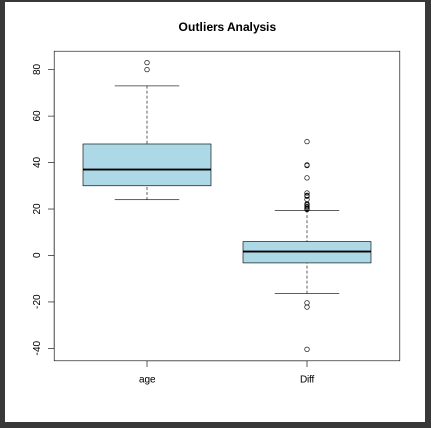
\includegraphics[width=0.5\linewidth]{part01_figures/1.png}
                    \caption{Visualize các biến `Age` và `Diff`}
                    \label{fig:Visualize các biến `Age` và `Diff`}
                \end{figure}
                Từ biểu đồ hộp, ta có nhận xét sau đây:
                    \begin{itemize}
                        \item \textbf{age}: Có một vài điểm cực ngoại lại ở phía trên.
                        \item \textbf{Diff}: Tồn tại nhiều điểm cực ngoại lai ở trên và ở phía dưới box.
                    \end{itemize}
        \end{itemize}
    \item [\textbf{Bước 4}]: \textbf{Trực quan hóa dữ liệu và rút ra nhận xét.}
    
        Ta sẽ dùng R để vẽ ra biểu đồ phân bố chuẩn của dữ liệu
        \begin{lstlisting}
# Biến Age
ggplot(islander_raw, aes(x = age)) +
  geom_histogram(aes(y = ..density..), bins = 30, color = "black", fill = "lightblue") +
  geom_density(alpha = 0.2, fill = "#FF6666") +
  stat_function(fun = dnorm, args = list(mean = mean(islander_raw$age, na.rm = TRUE), sd = sd(islander_raw$age, na.rm = TRUE)),
                color = "blue", size = 1) +
  theme_minimal() +
  labs(title = "Histogram of age variable", x = "age", y = "Density")

  # Biến Diff
  ggplot(islander_raw, aes(x = age)) +
  geom_histogram(aes(y = ..density..), bins = 30, color = "black", fill = "lightblue") +
  geom_density(alpha = 0.2, fill = "#FF6666") +
  stat_function(fun = dnorm, args = list(mean = mean(islander_raw$age, na.rm = TRUE), sd = sd(islander_raw$age, na.rm = TRUE)),
                color = "blue", size = 1) +
  theme_minimal() +
  labs(title = "Histogram of age variable", x = "age", y = "Density")
        \end{lstlisting}
            \begin{figure}[H]
                \centering
                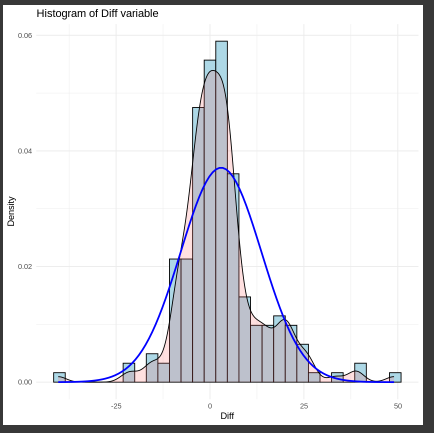
\includegraphics[width=0.3\linewidth]{part01_figures/2.png}
                \caption{Đồ thị phân phối chuẩn của biến `Diff`}
                \label{fig:Đồ thị phân phối chuẩn của biến `Diff`}
            \end{figure}
            \begin{figure}[H]
                \centering
                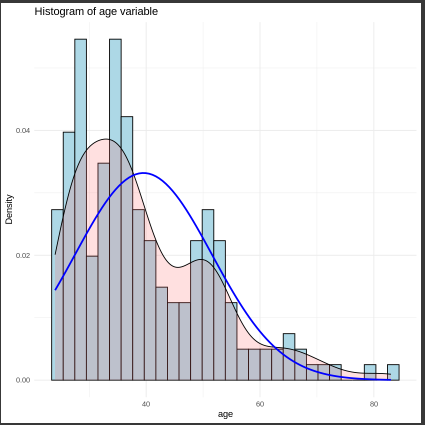
\includegraphics[width=0.3\linewidth]{part01_figures/3.png}
                \caption{Đồ thị phân phối chuẩn của biến `Age`}
                \label{fig:Đồ thị phân phối chuẩn của biến `Age`}
            \end{figure}
        Từ hai đồ thị trên, ta có một số nhận xét như sau:
            - `Age`: Không có dạng phân bố chuẩn, lệch trái so với giá trị trung bình
            - `Diff`: Có dạng phân bố gần chuẩn.
    \item [\textbf{Bước 4}]: \textbf{Kết luận}
    
    Sau khi hoàn thành bước khảo sát dữ liệu, ta có một số kết luận như sau
    \begin{itemize}
        \item [-] Các biến first-name và last-name chứa thông tin về tên của người khảo sát (kiểu dữ liệu character), về mặt thống kê biến này không có ý nghĩa nên sẽ được loại bỏ khỏi dữ liệu khi khảo sát.
        \item[-]  Vì Diff = Mem-Score-Before - Mem-Score-After (đa cộng tuyến), vì vậy ta chỉ cần khảo sát biến phụ thuộc Diff, các biến còn lại sẽ loại bỏ ra khỏi dữ liệu trước khi khảo sát.
        \item[-] Trên thực tế, việc khảo sát trên từng mức nhóm tuổi trải rộng từ 24 đến 83 rất nhiều, ta sẽ tiến hành chia thành 2 nhóm chính là nhóm tuổi < 50 và nhóm còn lại.
        \item[-] Biến phụ thuộc là `Diff` và các biến độc lập bao gồm  HappySadgroup, Dosage, Drug và age. 
    \end{itemize}
\end{itemize}

\subsection{Xử lý dữ liệu}
Ở bước này, chúng ta sẽ tiến hành các bước sau:
\begin{itemize}
    \item [1.] Loai bỏ các biến dư thừa và đưa dữ liệu về dạng thích hợp
    \item [2.] Xây dựng mô hình AOV để xem xét sự phụ thuộc của biến phụ thuộc vào các biến độc lập. Từ đó chọn ra các biến phù hợp để phân tích.
    \item [3.] Visualize các biến cần phân tích theo nhóm và rút ra nhận xét.
\end{itemize}
Sau đây là chi tiết các bước:
\begin{itemize}
    \item \textbf{Bước 1: Loại bỏ các biến cần thiết và asFactor các biến dạng category về dạng factor}

    \begin{lstlisting}
# Remove unesscessary variables
processed_islander = islander_raw[, !(names(islander_raw) %in% c("first_name", "last_name", "Mem_Score_Before", "Mem_Score_After"))]

processed_islander$age = processed_islander$age >= 50
processed_islander$age = factor(processed_islander$age)
processed_islander$Dosage = factor(processed_islander$Dosage)
processed_islander$Drug = factor(processed_islander$Drug)
processed_islander$Happy_Sad_group = factor(processed_islander$Happy_Sad_group)
levels(processed_islander$age)
levels(processed_islander$Drug)
levels(processed_islander$Dosage)
levels(processed_islander$Happy_Sad_group)
    \end{lstlisting}

    Kết quả thu được như sau:
\newpage
\begin{lstlisting}
'FALSE''TRUE'
'A''S''T'
'1''2''3'
'H''S'
\end{lstlisting}

    Kết quả cho ta thấy rằng nhóm tuổi đưọc chia thành 2 nhóm là trước 50 tuổi và từ 50 tuổi trở về sau, có 3 nhóm thuốc là A, S, T; có 3 liều lượng thuốc được sử dụng là 1, 2, 3 tương ứng với thấp, trung bình và cao; số người khảo sát nằm trong 2 nhóm là Happy và Sad (H, S).  


\item \textbf{Bước 2: Xây dựng mô hình AOV để xem xét sự phụ thuộc của biến phụ thuộc vào các biến độc lập như thế nào}
    \begin{lstlisting}
diff_aov = aov(Diff~., data = processed_islander)
summary(diff_aov)
    \end{lstlisting}

    Kết quả
    \begin{lstlisting}
                Df Sum Sq Mean Sq F value   Pr(>F)    
age               1      2     2.1   0.024  0.87821    
Happy_Sad_group   1     11    10.6   0.117  0.73233    
Dosage            2   1222   610.8   6.787  0.00142 ** 
Drug              2   4361  2180.6  24.229 4.19e-10 ***
Residuals       191  17190    90.0                     
---
Signif. codes:  0 '***' 0.001 '**' 0.01 '*' 0.05 '.' 0.1 ' ' 1
    \end{lstlisting}
    Nhìn vào bảng kết quả, ta thấy rằng thực tế các biến `HappySadgroup` và `age` không tham gia vào quá trình giải thích ý nghĩa của biến phụ thuộc `Diff` (với mức ý nghĩa 5\%). Do đó, ta chỉ chọn 2 biến `Drug` và `Dosage` để tiến hành khảo sát. Vậy:
    
    - \textbf{Mục tiêu}: Khảo sát về tác dụng phụ của các loại thuốc chống trầm cảm đối với trí nhớ của người tham gia thử nghiệm, được đánh giá thông qua thời gian hoàn thành một bài kiểm tra trí nhớ

    - \textbf{Biến phản hồi}: `Diff` cho biết chênh lệch giữa thời gian (giây) hoàn thành bài kiểm tra trước và sau khi sử dụng thuốc.
    
    - \textbf{Biến nhân tố}: \textbf{Drug}: Gồm 3 nhóm `A` (Alprazolam), `S` (Placebo) và `T` (Triazolam) và \textbf{Dosage}: Gồm 3 nhóm `1` (thấp), `2` (trung bình) và `3` (Cao)

    \item \textbf{Bước 3: Visualize dữ liệu của các biến theo từng nhóm}
    \begin{lstlisting}
processed_islander = processed_islander[, !(names(processed_islander) %in% c("age", "Happy_Sad_group"))]
# Dosage variable
ggplot(processed_islander ,aes(x=Dosage, y=Diff, colour=Dosage, fill=Dosage))+
  geom_jitter(width=0.25)+
  geom_boxplot(alpha=0.25, outlier.alpha=0) +
  stat_summary(fun.y=mean, colour="black", geom="point",
               shape=18, size=3,show.legend = FALSE) +
  theme_classic() +
  theme(legend.position="none")+
  theme(axis.text = element_text(angle=30, hjust=1, vjust=1))

#  Drug variable
ggplot(processed_islander ,aes(x=Drug, y=Diff, colour=Drug,fill=Drug))+
  geom_jitter(width=0.25)+
  geom_boxplot(alpha=0.25, outlier.alpha=0) +
  stat_summary(fun.y=mean, colour="black", geom="point",
               shape=18, size=3,show.legend = FALSE)+
  theme_classic()+
  theme(legend.position="none")+
  theme(axis.text = element_text(angle=30, hjust=1, vjust=1))
    \end{lstlisting}

Kết quả ta thu được như sau:
    \begin{figure}[H]
        \centering
        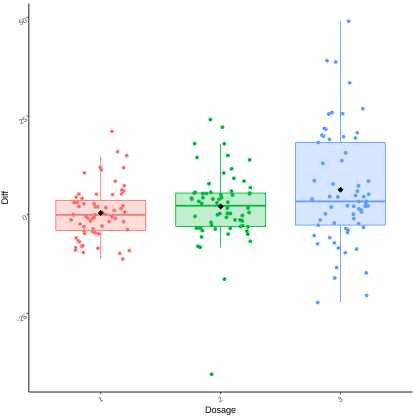
\includegraphics[width=0.4\linewidth]{part01_figures/4.png}
        \caption{Phân phối dữ liệu của từng nhóm Dosage}
        \label{fig:Phân phối dữ liệu của từng nhóm Dosage}
    \end{figure}
    \begin{figure}[H]
        \centering
        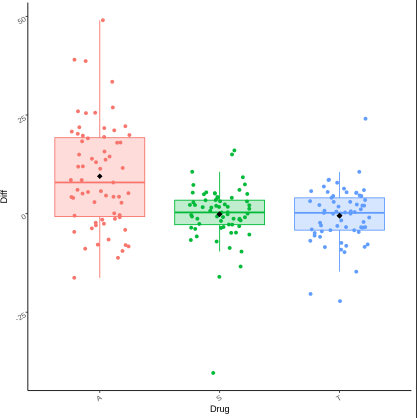
\includegraphics[width=0.4\linewidth]{part01_figures/5.png}
        \caption{Phân phối dữ liệu của từng nhóm Drug}
        \label{fig:Phân phối dữ liệu của từng nhóm Drug}
    \end{figure}

    Nhìn vào đây, ta có thể rút ra một vài nhận xét như sau:
    \begin{itemize}
        \item Đối với Dosage
        \begin{itemize}
            \item Liều lượng thấp: Trung vị Diff gần bằng 0, với phạm vi nhỏ. Hầu hết các điểm dữ liệu tập trung xung quanh trung vị, với một vài ngoại lệ.
            \item Liều lượng trung bình: Trung vị Diff vẫn gần bằng 0, nhưng phạm vi dữ liệu lớn hơn một chút so với liều lượng thấp. Có sự phân bố rộng hơn của các điểm, cho thấy sự biến đổi nhiều hơn trong các phản ứng.
            \item  Liều lượng cao: Trung vị Diff cao hơn so với các nhóm khác, gợi ý rằng liều lượng thuốc này có tác dụng lớn hơn. Có sự biến đổi lớn, với một số điểm nằm khá cao hoặc thấp so với trung vị.IQR lớn hơn và sự hiện diện của các ngoại lệ cho thấy một phạm vi rộng của các phản ứng đối với liều lượng cao.
        \end{itemize}
        Ta rút ra kết luận như sau:
            \begin{itemize}
                \item Biểu đồ gợi ý rằng liều lượng cao hơn có thể có tác động đáng kể hơn đến thời gian hoàn thành bài kiểm tra trí nhớ, được chỉ ra bởi trung vị cao hơn và sự biến đổi lớn hơn trong Diff.
                \item Liều lượng thấp và trung bình cho thấy sự thay đổi nhỏ hơn và ít biến đổi hơn, với nhiều người tham gia có ít hoặc không thay đổi trong thời gian hoàn thành.
                \item Sự phân bố rộng hơn và trung vị cao hơn trong nhóm liều lượng cao có thể cho thấy rằng mặc dù một số người tham gia có lợi ích đáng kể, những người khác có thể gặp tác dụng phụ, dẫn đến phản ứng không tốt.

            \end{itemize}
        \item  Đối với Drug
        \begin{itemize}
            \item Alprazolam (A):Trung vị Diff khá xa với điểm 0 hơn các loại thuốc khác.Có nhiều điểm ngoại lệ, đặc biệt ở phía trên, cho thấy một số người tham gia có sự cải thiện đáng kể về thời gian hoàn thành bài kiểm tra.Trung bình Diff cũng cao hơn, gợi ý rằng Alprazolam có thể có tác dụng tích cực đối với một số người tham gia.

            \item Triazolam (T):Trung vị Diff gần bằng 0, với phạm vi và sự phân tán nhỏ hơn so với Alprazolam. Trung bình Diff gần với trung vị, cho thấy tác dụng của Triazolam ít biến đổi hơn.
            \item Placebo (S):Trung vị Diff gần bằng 0, với phạm vi và sự phân tán tương tự như Triazolam. Có một số điểm ngoại lệ, nhưng không nhiều.Trung bình Diff gần với trung vị, cho thấy tác dụng của giả dược (Placebo) ít biến đổi và không có hiệu quả đáng kể.
        \end{itemize}
        Ta rút ra kết luận như sau:
        \begin{itemize}
            \item Alprazolam (A): Có tác dụng đáng kể đối với một số người tham gia, nhưng cũng có nhiều biến đổi, cho thấy có thể có tác dụng phụ hoặc tác động không đồng nhất.
            \item  Triazolam (T) và Placebo (S): Không có sự thay đổi đáng kể trong thời gian hoàn thành bài kiểm tra, gợi ý rằng các loại thuốc này có ít hoặc không có tác dụng cải thiện trí nhớ.
        \end{itemize}
    \end{itemize}

    Ta xem xét biến phụ thuộc Diff bằng cách xét lại biểu đồ phân bố chuẩn như sau:
    \begin{lstlisting}
ggplot(processed_islander, aes(x = Diff)) +
  geom_histogram(aes(y = ..density..), bins = 30, color = "black", fill = "lightblue") +
  geom_density(alpha = 0.2, fill = "#FF6666") +
  stat_function(fun = dnorm, args = list(mean = mean(processed_islander$Diff, na.rm = TRUE), sd = sd(processed_islander$Diff, na.rm = TRUE)),
                color = "blue", size = 1) +
  theme_minimal() +
  labs(title = "Histogram of Diff variable", x = "Diff", y = "Density")
    \end{lstlisting}
    \begin{figure}[H]
                \centering
                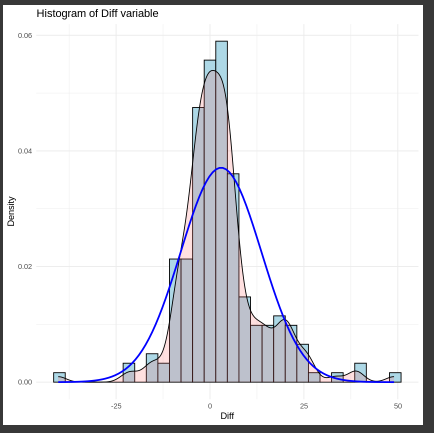
\includegraphics[width=0.8\linewidth]{part01_figures/2.png}
                \caption{Đồ thị phân phối chuẩn của biến `Diff`}
                \label{fig:Đồ thị phân phối chuẩn của biến `Diff`_}
            \end{figure}
    Ta cũng rút ra một vài nhận xét như sau:
    \begin{itemize}
        \item Độ lệch
        \begin{itemize}
            \item Trung bình (Mean) của biến Diff là 2.955, cho thấy thời gian trung bình hoàn thành bài kiểm tra sau khi dùng thuốc tăng thêm khoảng 2.955 giây.
            \item Median (Trung vị) là 1.700, thấp hơn giá trị trung bình, cho thấy sự phân phối không hoàn toàn đối xứng.
        \end{itemize}
        \item Phân Bố Dữ Liệu: Dữ liệu phân bố khá gần với phân phối chuẩn, nhưng có một vài khác biệt:
        \begin{itemize}
            \item Có một sự tập trung dữ liệu khá cao xung quanh giá trị 0 đến 5, tạo nên một đỉnh phân phối cao hơn so với đường chuẩn.
            \item Có sự lan tỏa dữ liệu về cả hai phía của đỉnh, nhưng ít hơn ở phía cực trái (khoảng -40) và cực phải (khoảng 50).
        \end{itemize}

        \item Khoảng Tứ Phân Vị:
        \begin{itemize}
            \item 1st Qu. (Quartile đầu tiên): -3.175.
            \item 3rd Qu. (Quartile thứ ba): 5.925.
            \item Điều này cho thấy phần lớn dữ liệu nằm trong khoảng từ -3.175 đến 5.925, một khoảng phân tán rộng nhưng không đối xứng hoàn toàn quanh trung vị.
        \end{itemize}
        \item  Đỉnh và đuôi: Biểu đồ cho thấy một đỉnh lớn, khá hẹp, và hai đuôi phân phối khá dài, đặc biệt ở phía phải (hơn 25). Điều này chỉ ra rằng có một số giá trị cực đại cao (tăng lớn trong thời gian hoàn thành bài kiểm tra sau khi dùng thuốc).
    \end{itemize}
    \newpage
    Kết Luận:
    \begin{itemize}
        \item Sự Phân Tán và Độ Lệch: Biểu đồ cho thấy sự tăng thời gian hoàn thành bài kiểm tra (Diff) sau khi dùng thuốc là phổ biến, với giá trị trung bình dương. Tuy nhiên, phân phối không hoàn toàn đối xứng, với một số giá trị cực đại ở cả hai phía.
        \item Khả Năng Phân Phối Chuẩn: Phân phối của biến Diff khá gần với phân phối chuẩn, nhưng có một số khác biệt như đỉnh phân phối cao hơn và đuôi phân phối dài hơn. Điều này có thể là do tác động của một số cá nhân phản ứng mạnh mẽ với thuốc hơn so với phần còn lại.
    \end{itemize}
\end{itemize}

\subsection{Kiểm định các giả thiết thống kê (ANOVA assumptions)}
Nhắc lại các điều kiện để phân tích ANOVA như sau:
\begin{itemize}
    \item [1.] Các mẫu độc lập
    \item [2.] Biến phụ thuộc là biến liên tục
    \item [3.] Các nhóm có phân phối chuẩn hoặc gần chuẩn, đồng nghĩa với việc kiểm định phương sai các nhóm cho kết quả là đồng nhất.
\end{itemize}

Rõ ràng, theo như phân tích phía trên, bộ dữ liệu chúng ta đã thỏa mãn điều kiện (1) và (2). Để chắc chắn ta sẽ đi kiểm định yêu cầu số (3) bằng cách tiến hành thực hiện các kiểm định sau:
\begin{itemize}
    \item Shapiro-Wilk test
    \item leveneTest
    \item durbinWatsonTest
\end{itemize}

Đầu tiên ta sẽ xây dựng mô hình tương tác bằng dòng lệnh sau
\begin{lstlisting}
# Xây dựng mô hình tương tác
int_model = aov(Diff~Dosage * Drug, data = processed_islander)
summary(int_model)
\end{lstlisting}

Kết quả thu được:

\begin{lstlisting}
                 Df Sum Sq Mean Sq F value   Pr(>F)    
Dosage        2   1222   610.9   9.536 0.000113 ***
Drug          2   4314  2156.9  33.666 3.12e-13 ***
Dosage:Drug   4   5141  1285.3  20.062 8.74e-14 ***
Residuals   189  12109    64.1                     
---
Signif. codes:  0 '***' 0.001 '**' 0.01 '*' 0.05 '.' 0.1 ' ' 1
\end{lstlisting}
Với mức ý nghĩa 5\%, ta thấy rằng giữa `Dosage` và `Drug` có mối quan hệ tương tác với nhau dẫn đến tác động hiệu quả của việc dùng thuốc đối với trí nhớ của người sử dụng. Tiếp tục đi kiểm định các thông số sau:

\begin{lstlisting}
# Shapiro-Wilk test
int_model = aov(Diff~Dosage * Drug, data = processed_islander)
av_residual = rstandard(int_model)
shapiro.test(av_residual)
# QQ plot
qqnorm(av_residual)
qqline(av_residual)
hist(av_residual)
\end{lstlisting}

\begin{figure}[H]
    \centering
    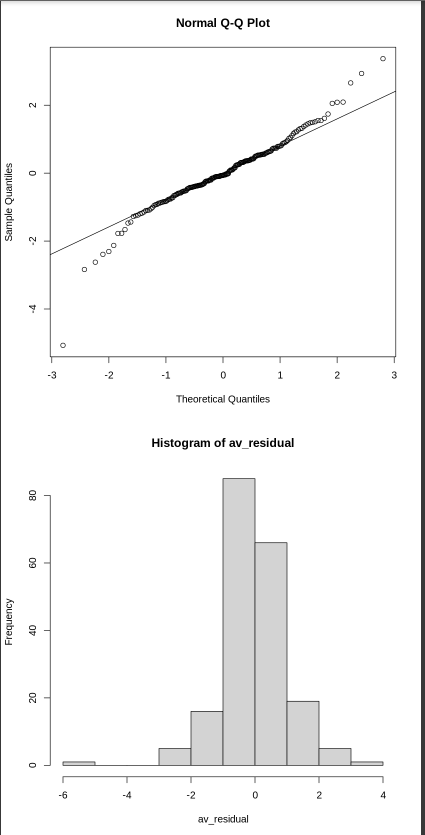
\includegraphics[width=0.45\linewidth]{part01_figures/6.png}
    \caption{Biểu đồ phần dư}
    \label{fig:Biểu đồ phần dư}
\end{figure}

\newpage
Kết quả như sau:
\begin{lstlisting}
    	Shapiro-Wilk normality test

data:  av_residual
W = 0.95575, p-value = 7.794e-06
\end{lstlisting}

Xét giả định
\begin{itemize}
    \item H0: Tuân theo phân phối chuẩn
    \item H1: Không tuân theo phân phối chuẩn
\end{itemize}

Nhận xét: Với độ tin cậy 5\% thì với giá trị p-value = 7.794e-06 chúng ta đủ cơ sở bác bỏ H0, vậy phần dư có phân phối không chuẩn. Nhìn vào biểu đồ, ta thấy rằng ở phần đuôi kéo dài, có một vài điểm bị kéo lệch ra khỏi đường thẳng, điều này chứng tỏ rằng khả năng các điểm nhiễu chính là các điểm ngoại lệ (outliners), tuy nhiên, về mặt tổng quan, dữ liệu vẫn có dạng gần chuẩn, do đó, ta vẫn có thể tiến hành kiểm tra ANOVA. Ở bước cải tiến, ta sẽ tiến hành xử lý các điểm ngoại lệ này để so sánh với kiểm định ban đầu.

Bước tiếp theo ta Kiểm định các nhóm có phương sai đồng nhất hay không
\begin{lstlisting}
leveneTest(int_model)
\end{lstlisting}

Kết quả
\begin{lstlisting}
Df	F value	Pr(>F)
<int>	<dbl>	<dbl>
group	8	0.9961061	0.4404991
189	NA	NA
\end{lstlisting}

Giả định:

- H0: Các nhóm có phương sai đồng nhất

- H1: Các nhóm không có phương sai đồng nhất

Nhận xét: Với giá trị p-value = 0.4404991 > 0.05, ta không đủ điều kiện bác bỏ H0, vậy các nhóm có phương sai đồng nhất. Như vậy, bộ dữ liệu này đã thoả mãn điều kiện yêu cầu để phân tích ANOVA. Tuy nhiên, để hiểu sâu hơn về bộ dữ liệu, ta tiếp tục đi kiểm định tính độc lập của phần dư bằng dòng lệnh sau

\newpage
\begin{lstlisting}
# Kiểm định tính độc lập của phần dư
durbinWatsonTest(int_model)
plot(int_model, 1)
\end{lstlisting}

Kết quả 
\begin{lstlisting}
 lag Autocorrelation D-W Statistic p-value
   1     -0.05315976      2.105716   0.816
 Alternative hypothesis: rho != 0

\end{lstlisting}
\begin{figure}[H]
    \centering
    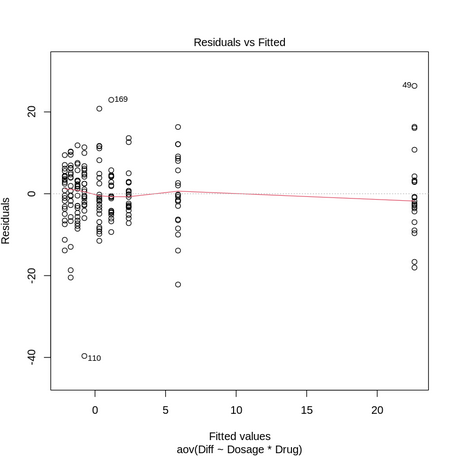
\includegraphics[width=0.8\linewidth]{part01_figures/7.png}
    \caption{Kiểm định độc lập phần dư}
    \label{fig:Kiểm định độc lập phần dư}
\end{figure}
Với giả định:
\begin{itemize}
    \item H0: Không có sự tương quan (độc lập).
    \item H1: H1: Có sự tương quan (không độc lập).
\end{itemize}

Thì với giá trị p-value = 0.816 (> 0.05) nên không có sự tương quan. Vậy phần dư độc lập

\subsection{Phân tích phương sai k nhân tố}
Tiếp theo chung ta sẽ tiến hành đi phân tích phương sai k nhân tố. Việc này gồm các bước sau:
\begin{itemize}
    \item [1.] Kiểm tra sự tương tác
    \item [2.] Phân tích ảnh hưởng đơn
    \begin{itemize}
        \item Phân tích ảnh hưởng đơn của liều lượng ở mỗi loại thuốc
        \item Phân tích ảnh hưởng đơn của thuốc ở mỗi liều lượng
    \end{itemize}
    \item [3.] Phân tích ảnh hưởng chính
    \begin{itemize}
        \item Phân tích ảnh hưởng chính của Dosage với hiệu quả của bài kiểm tra trí nhớ
        \item Phân tích ảnh hưởng chính của Drug với hiệu quả của bài kiểm tra trí nhớ
    \end{itemize}
\end{itemize}

Sau đây là các bước chi tiết:
\begin{itemize}
    \item \textbf{Bước 1: Xây dựng mô hình tương tác (interaction model) và kiểm tra tương tác của các biến}

    \begin{lstlisting}
    int_model = aov(Diff~Dosage * Drug, data = processed_islander)
    summary(int_model)
    plot(interactionMeans(int_model))
    \end{lstlisting}

    Kết quả
    \begin{lstlisting}
                     Df Sum Sq Mean Sq F value   Pr(>F)    
Dosage        2   1222   610.9   9.536 0.000113 ***
Drug          2   4314  2156.9  33.666 3.12e-13 ***
Dosage:Drug   4   5141  1285.3  20.062 8.74e-14 ***
Residuals   189  12109    64.1                     
---
Signif. codes:  0 '***' 0.001 '**' 0.01 '*' 0.05 '.' 0.1 ' ' 1
    \end{lstlisting}
Ta rút ra một số nhận xét dựa trên kết quả như sau: 

- Với mức ý nghĩa 5\%, ta thấy giữa `Dosage` và `Drug` có sự tương tác với nhau (p-value=8.74e-14). Sự kết hợp giữa hàm lượng thuốc và loại thuốc có ảnh hưởng rất lớn đến thời gian hoàn thành bài kiểm tra, cho thấy rằng không chỉ từng yếu tố riêng lẻ mà sự kết hợp giữa chúng cũng rất quan trọng.

- Đối với biểu đồ bên trái: Biểu đồ bên trái biểu diễn sự tương tác giữa Dosage và Drug dựa trên giá trị trung bình điều chỉnh của Diff.
    \begin{itemize}
        \item [+]  Đồ thị trên cùng bên trái (Dosage theo Drug):
        \begin{itemize}
            \item Cho thấy sự thay đổi của Diff theo liều lượng (Dosage) cho từng loại thuốc (Drug).
            \item Đối với tất cả các loại thuốc, Diff tăng dần khi tăng liều lượng từ 1 đến 3.
        \end{itemize}
        \item [+]  Đồ thị dưới cùng bên trái (Drug theo Dosage):
        \begin{itemize}
            \item Cho thấy sự thay đổi của Diff theo loại thuốc (Drug) cho từng liều lượng (Dosage).
            \item Khi liều lượng là 1: sự khác biệt giữa các loại thuốc là tương đối nhỏ. Trong đó loại S cho hiệu quả cao nhất, A và T cho kết quả tệ hơn trước khi sử dụng (mean < 0).
            \item Khi liều là 2: Có sự thay đổi rõ rệt ở các loại thuốc: Loại S cho kết quả tệ hơn so với trước khi dùng thuốc, loại T có hiệu quả không đáng kể, loại A cho thấy hiệu quả vượt bật.
            \item Khi liều lượng là 3: Sự khác biệt giữa các loại thuốc trở nên rõ rệt hơn, với Thuốc A cho kết quả tốt nhất so với 3 loại và ở cả 3 liều lượng, trong khi 2 loại còn lại cho kết quả tệ hơn trước khi dùng.
        \end{itemize}
    \end{itemize}

- Đối với biểu đồ bên phải: Biểu đồ bên phải biểu diễn sự tương tác giữa Drug và Dosage dựa trên giá trị trung bình điều chỉnh của Diff.
    \begin{itemize}
        \item [+] Đồ thị trên cùng bên phải (Drug theo Dosage):
        \begin{itemize}
            \item Tương tự như đồ thị dưới cùng bên trái của biểu đồ bên trái, nhưng theo chiều ngược lại. Cho thấy sự thay đổi của Diff theo loại thuốc cho từng liều lượng.
            \item Đối với thuốc A: Cho kết quả tốt liều lượng cao và trung bình, liều lượng thấp không có sự thay đổi
            \item Đối với thuốc T: Không có sự khác biệt giữa các liều lượng và hiệu quả sau và trước khi sửng dụng (Thậm chí giảm (tệ))
            \item Đối với thuốc S: Giống T
        \end{itemize}
        \item [+] Đồ thị dưới cùng bên phải (Dosage theo Drug):
        \begin{itemize}
            \item Tương tự như đồ thị trên cùng bên trái của biểu đồ bên trái, nhưng theo chiều ngược lại.
            \item Cho thấy sự thay đổi của Diff theo liều lượng cho từng loại thuốc.
            \item Cơ bản các thuốc cho kết quả tốt nhất theo thứ tự là là A > S > T.
        \end{itemize}
    \end{itemize}
Ta có kết luận sau đây:
    \begin{itemize}
        \item Cả liều lượng và loại thuốc đều có ảnh hưởng đáng kể đến Diff.
        \item Có sự tương tác đáng kể giữa liều lượng và loại thuốc, nghĩa là hiệu quả của liều lượng khác nhau phụ thuộc vào loại thuốc được sử dụng.
        \item Biểu đồ cho thấy rõ ràng rằng Thuốc A (Alprazolam) có ảnh hưởng lớn nhất khi liều lượng tăng, trong khi S có ảnh hưởng ít nhất.
    \end{itemize}

\item \textbf{Bước 2: Phân tích ảnh hưởng đơn}

        Để phân tích ảnh hưởng đơn ta sẽ sử dụng hàm \textbf{testInteractions} để tiến hành phân tích. Sau đây là các bước chi tiết
    \begin{itemize}
        \item Phân tích ảnh hưởng đơn của liều lượng ở mỗi loại thuốc
            \begin{lstlisting}
testInteractions(int_model, fixed = "Drug", across = "Dosage")
            \end{lstlisting}
            Kết quả:
            \begin{figure}[H]
                \centering
                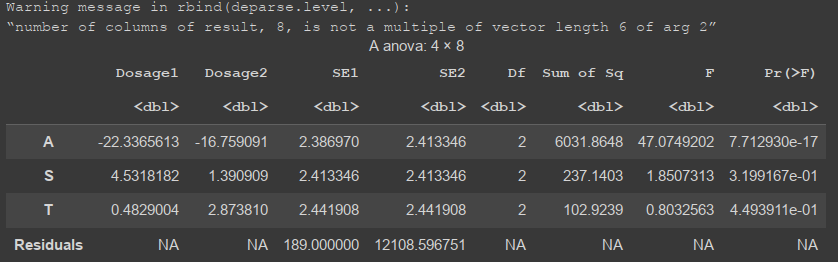
\includegraphics[width=0.8\linewidth]{part01_figures/8.png}
                \caption{Kết quả ảnh hưởng đơn giữa Drug và Dosage}
                \label{fig:Kết quả ảnh hưởng đơn giữa Drug và Dosage}
            \end{figure}
            Với các giả định như sau:
            \begin{itemize}
                \item H0: Liều lượng không ảnh hưởng đến hiệu quả thuốc
                \item H1: Liều lượng có ảnh hưởng đến hiệu quả của thuốc
            \end{itemize}
            Ta rút ra kết luận như sau: Với kết quả phân tích ta có một số nhận xét như sau, với độ tin cậy 5\% thì:
            \begin{itemize}
                \item Liều lượng có ảnh hưởng đến kết quả của loại thuốc A
                \item Liều lượng không ảnh hưởng đến kết quả của lọa thuốc S và T
            \end{itemize}
        \item Phân tích ảnh hưởng đơn của thuốc ở mỗi liều lượng
            \begin{lstlisting}
    testInteractions(int_model, fixed = "Dosage", across = "Drug")
            \end{lstlisting}
            \begin{figure}[H]
                \centering
                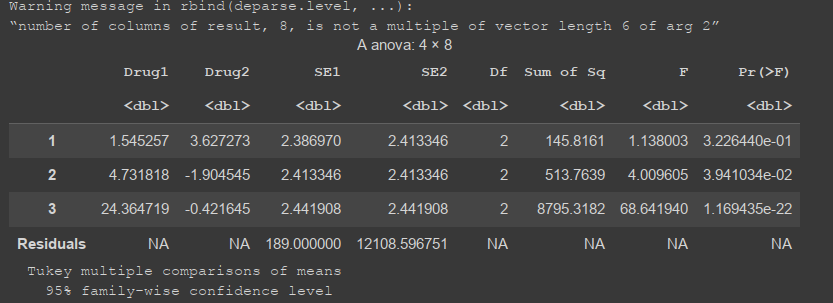
\includegraphics[width=0.8\linewidth]{part01_figures/9.png}
                \caption{Ảnh hưởng đơn giữa Drug và Dosage.}
                \label{fig:Ảnh hưởng đơn giữa Drug và Dosage.}
            \end{figure}
            Tương tự như ở phía trên, ta có các giả định như sau:
            \begin{itemize}
                \item H0: Các loại thuốc sẽ không tác động ở mỗi liều lượng
                \item H1: Các loại thuốc sẽ có tác động ở mỗi liều lượng
            \end{itemize}
        Ta rút ra kết luận như sau: Với kết quả phân tích ta có một số nhận xét như sau, với độ tin cậy 5\% thì:
            \begin{itemize}
                \item Hầu hết các loại thuốc sẽ có tác động ở liều lượng cao
                \item Liều lượng trung bình cũng sẽ có tác động nhưng không đáng kể (có ý nghĩa ở mức 0.4%)
                \item Liều lượng thấp cho kết quả không đáng kể.
            \end{itemize}
        \item Phân tích ảnh hưởng đơn giữa các nhóm thuốc ứng với mỗi liều lượng
        
        Việc phân tích sự tương tác của các nhóm trong cùng một liều lượng cũng có ý nghĩa rất quan trọng trong thống kê, từ đó sẽ hiểu rõ hơn về từng tác dụng của từng loại và từng nhóm
        \begin{lstlisting}
options(contrasts = c(unordered="contr.sum", ordered="contr.poly"))
A_vs_S = list(Drug = c(1, -1, 0))
A_vs_T = list(Drug = c(1, 0, -1))
S_vs_T = list(Drug = c(0, 1, -1))
        \end{lstlisting}

        Đầu tiên, ta sẽ đi phân tích ảnh hưởng của nhóm A và S
        \begin{lstlisting}
testInteractions(int_model, custom = c(A_vs_S), fixed = "Dosage", adjustment = "bonferroni")
        \end{lstlisting}
        Kết quả:
        \begin{figure}[H]
            \centering
            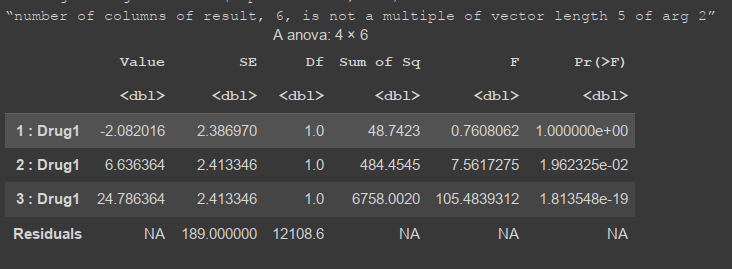
\includegraphics[width=0.8\linewidth]{part01_figures/10.png}
            \caption{Tương tác giữa nhóm A và S ở mỗi liều lượng}
            \label{fig:Tương tác giữa nhóm A và S ở mỗi liều lượng}
        \end{figure}
        Ta có giả định như sau:
        \begin{itemize}
            \item Không có sự khác nhau giữa nhóm thuốc A và S ở các liều lượng
            \item Có sự khác nhau giữa nhóm thuốc A và S ở các liều lượng
        \end{itemize}
        Ta rút ra kết luận như sau: Với kết quả phân tích ta có một số nhận xét như sau, với độ tin cậy 5\% thì:
        \begin{itemize}
            \item Có sự khác biệt về hiệu quả khi sử dụng thuốc thuốc A và S ở các  liều lượng cao và trung bình
            \item Ở liều lượng thấp: Không có sự khác biệt
        \end{itemize}

        Tiếp theo là nhóm A và T
        
        \begin{lstlisting}
testInteractions(int_model, custom = c(A_vs_T), fixed = "Dosage", adjustment = "bonferroni")
        \end{lstlisting}
        Kết quả:
        \begin{figure}[H]
            \centering
            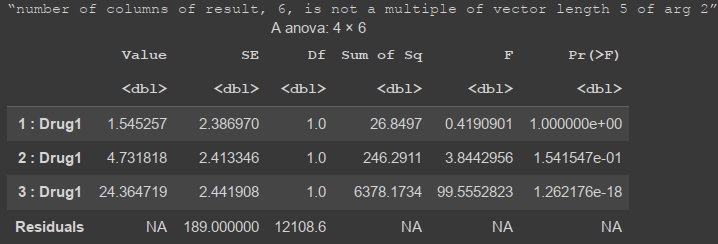
\includegraphics[width=0.8\linewidth]{part01_figures/11.png}
            \caption{Tương tác giữa nhóm A và T ở mỗi liều lượng}
            \label{fig:Tương tác giữa nhóm A và T ở mỗi liều lượng}
        \end{figure}
        Với các giả định tương tự với nhóm A và S, ta có kết luận như sau:
        \begin{itemize}
            \item Ở liều cao: Có sự khác biệt về hiệu quả khi sử dụng thuốc ở các  loại thuốc A và T
            \item Ở liều thấp và trung bình: Không có sựu ảnh hưởng rõ rệt
        \end{itemize}
        Cuối cùng là giữa nhóm S và T
        \begin{lstlisting}
testInteractions(int_model, custom = c(S_vs_T), fixed = "Dosage", adjustment = "bonferroni")
        \end{lstlisting}
        Kết quả:
        \begin{figure}[H]
            \centering
            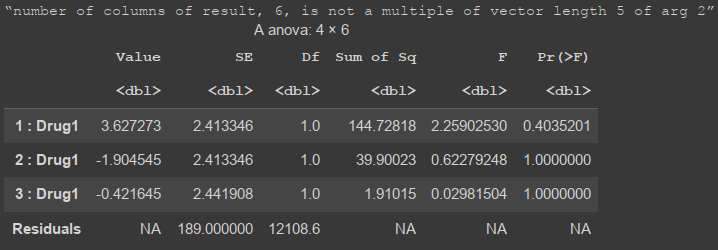
\includegraphics[width=0.8\linewidth]{part01_figures/12.png}
            \caption{Tương tác giữa nhóm S và T ở mỗi liều lượng}
            \label{fig:Tương tác giữa nhóm S và T ở mỗi liều lượng}
        \end{figure}
         Với các giả định tương tự với nhóm A và S, ta có kết luận như sau: Với độ tin cậy 5\% thì không có sự khác biệt nào ở cả 3 liều lượng.
    \end{itemize}
    Từ việc phân tích trên, ta có kết luận như sau: Khi dùng thuốc liều cao, giữa các nhóm sẽ cho ra các phản ứng ảnh hưởng đến trí nhớ ở nhóm A-T và A-S. Tuy nhiên, nhóm S-T lại không cho thấy sự tương tác nào có ý nghĩa thống kê.

    \item Phân tích ảnh hưởng đơn giữa các nhóm liều lượng ứng với mỗi loại thuốc
    Tương tự cho trường hợp \textbf{Phân tích ảnh hưởng đơn giữa các nhóm thuốc ứng với mỗi liều lượng}, ta cũng phân tích ảnh hưởng đơn giữa các nhóm liều lượng ứng với mỗi loại thuốc như thế nào
    \begin{lstlisting}
options(contrasts = c(unordered="contr.sum", ordered="contr.poly"))
low_vs_medium = list(Dosage = c(1, -1, 0))
low_vs_high = list(Dosage = c(1, 0, -1))
medium_vs_high = list(Dosage = c(0, 1, -1))
    \end{lstlisting}
    Đầu tiên là nhóm thấp và trung bình
    \begin{lstlisting}
# Nhóm thấp và trung bình
testInteractions(int_model, custom = c(low_vs_medium), fixed = "Drug", adjustment = "bonferroni")
    \end{lstlisting}
    Kết quả:
    \begin{figure}[H]
        \centering
        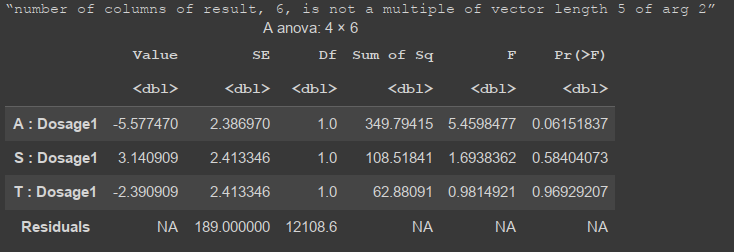
\includegraphics[width=0.8\linewidth]{part01_figures/13.png}
        \caption{Tương tác giữa nhóm thấp và nhóm trung bình}
        \label{fig:Tương tác giữa nhóm thấp và nhóm trung bình}
    \end{figure}
    Với giả định sau:
        \begin{itemize}
            \item H0: Không có sự tương tác nhau giữa liều thấp và liều trung bình ở loại thuốc X (A, T, S)
            \item H1: Có sự tương tác nhau giữa liều thấp và liều trung bình ở  ở loại thuốc X (A, T, S)
        \end{itemize}
    Với độ tin cậy 5\% thì
    \begin{itemize}
        \item Ở loại thuốc A: Có sự tương tác về hiệu quả khi sử dụng thuốc ở các  liều lượng thấp và liều lượng trung bình
        \item Ở loại thuốc S và T: Không có sự tương tác
    \end{itemize}

    Tiếp theo là nhóm thấp và cao
    \begin{lstlisting}
# Nhóm thấp và cao
testInteractions(int_model, custom = c(low_vs_high), fixed = "Drug", adjustment = "none")
    \end{lstlisting}
\begin{figure}[H]
    \centering
    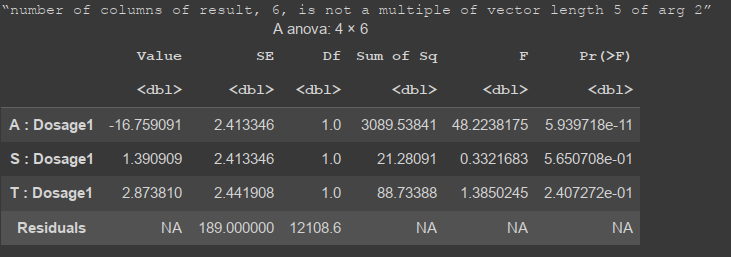
\includegraphics[width=0.8\linewidth]{part01_figures/14.png}
    \caption{Tương tác giữa nhóm thấp và cao}
    \label{fig:Tương tác giữa nhóm thấp và cao}
\end{figure}
    Tương tự như trên ta rút ra nhận xét như sau: Với mức ý nghĩa 5\%
    \begin{itemize}
        \item Ở loại thuốc A: Có sự tương tác khi sử dụng thuốc ở các liều lượng thấp và liều lượng cao
        \item Ở loại thuốc S và T: Không có sự tương tác mang ý nghĩ thống kê
    \end{itemize}

    Cuối cùng là nhóm trung bình và cao
    \begin{lstlisting}
# Nhóm trung bình và cao
testInteractions(int_model, custom = c(medium_vs_high), fixed = "Drug", adjustment = "none")
    \end{lstlisting}
\begin{figure}[H]
    \centering
    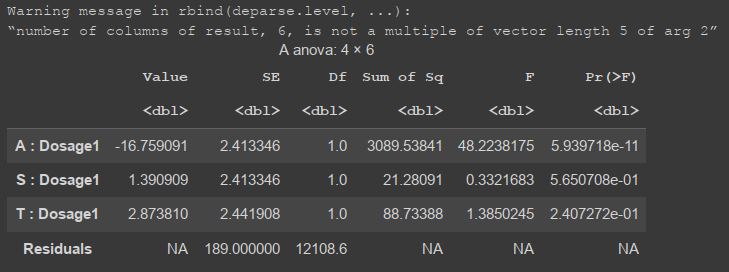
\includegraphics[width=0.8\linewidth]{part01_figures/15.png}
    \caption{Tương tác giữa nhóm trung bình và cao}
    \label{fig:Tương tác giữa nhóm trung bình và cao}
\end{figure}
    Tương tự như trên ta rút ra nhận xét như sau: Với mức ý nghĩa 5\%
    \begin{itemize}
        \item Có sự tương tác khi sử dụng thuốc ở các  liều lượng trung bình và liều lượng cao
        \item Không có sự tương tác mang ý nghĩa thống kê
    \end{itemize}

    Qua việc phân tích trên ta có một số kết luận như sau:
    \begin{itemize}
        \item Hầu hết các liều lượng thấp và trung bình sẽ cho thấy mức độ ít tương tác mang ý nghĩ thống kê ở các loại thuốc
        \item Hầu hết các loại thuốc T và S cho kết quả là không có sự tương tác giữa liều lượng với loại A
    \end{itemize}
    \item \textbf{Bước 3: Phân tích ảnh hưởng chính}

    Ở bước này ta sẽ thực hiện 2 phân tích:
    \begin{itemize}
        \item Phân tích ảnh hưởng chính của Dosage với hiệu quả của bài kiểm tra trí nhớ
        \item Phân tích ảnh hưởng chính của Drug với hiệu quả của bài kiểm tra trí nhớ
    \end{itemize}
    Với mỗi bước, ta sẽ thực hiện các công việc sau:
    \begin{itemize}
        \item Xây dựng mô hình
        \item Kiểm định các giả thiết của mô hình
        \item Kiểm định trung bình của các nhóm
        \item Nhận xét
    \end{itemize}
    Sau đây là các bước phân tích cụ thể:
    \begin{itemize}
        \item \textbf{Bước 3.1: Phân tích ảnh hưởng chính của Dosage với hiệu quả của bài kiểm tra trí nhớ}
        \begin{lstlisting}
dosage_model = aov(Diff~Dosage, data = processed_islander)
summary(dosage_model)
        \end{lstlisting}
        Kết quả:
        \begin{lstlisting}
            Df Sum Sq Mean Sq F value  Pr(>F)   
Dosage        2   1222   610.9   5.524 0.00464 **
Residuals   195  21563   110.6                   
---
Signif. codes:  0 '***' 0.001 '**' 0.01 '*' 0.05 '.' 0.1 ' ' 1
        \end{lstlisting}
        Nhận xét: Với mức ý nghĩa 0.05, ta thấy rằng Dosage có ý nghĩa trong việc giải thích mô hình

        Tiếp theo tiến hành kiểm định các giả thuyết
        \begin{lstlisting}
# Shapiro-Wilk test
av_residual = rstandard(dosage_model)
shapiro.test(av_residual)

# Trực quan bằng QQ plot
qqnorm(av_residual)
qqline(av_residual)
hist(av_residual)
        \end{lstlisting}
        Kết quả:
        \begin{lstlisting}
    Shapiro-Wilk normality test

data:  av_residual
W = 0.94813, p-value = 1.397e-06
        \end{lstlisting}
        Với giả định:
        \begin{itemize}
            \item H0: Phần dư Tuân theo phân phối chuẩn.
            \item H1: Phần dư Không tuân theo phân phối chuẩn.
        \end{itemize}
        Như vậy với độ tin cậy 5\% thì với giá trị p-value = 1.397e-06 chúng ta đủ cơ sở bác bỏ H0, vậy sai số có phân phối không chuẩn. Nhìn vào biểu đồ, ta thấy rằng ở phần đuôi kéo dài, có một vài điểm bị kéo lệch ra khỏi đường thẳng --> Khả năng các điểm nhiễu chính là các điểm ngoại lệ (outliners), tuy nhiên, về mặt tổng quan, dữ liệu vẫn có dạng gần chuẩn.

    \begin{lstlisting}
# Kiểm định các nhóm có phương sai đồng nhất hay không
leveneTest(dosage_model)
    \end{lstlisting}
    Kết quả:
    \begin{lstlisting}
        A anova: 2 x 3 	
        Df	F value	Pr(>F)
	<int>	<dbl>	  <dbl>
group	2	11.76277   1.502826e-05
	   195	       NA	       NA
    \end{lstlisting}
    Với giả định:
    \begin{itemize}
        \item Các nhóm có phương sai đồng nhất.
        \item Các nhóm không có phương sai đồng nhất.
    \end{itemize}
    Nhận xét: Với giá trị p-value = 1.502826e-05 < 0.05, ta đủ điều kiện bác bỏ H0, vậy các nhóm có phương sai không đồng nhất.
    \end{itemize}
    \begin{lstlisting}
# Kiểm định tính độc lập của phần dư
durbinWatsonTest(dosage_model)
plot(dosage_model, 1)
    \end{lstlisting}
    Kết quả:
    \begin{lstlisting}
 lag Autocorrelation D-W Statistic p-value
   1       0.3993242      1.198467       0
 Alternative hypothesis: rho != 0        
    \end{lstlisting}
    Với giả định:
    \begin{itemize}
        \item H0: Không có sự tương quan (độc lập)
        \item H1: Có sự tương quan (không độc lập)
    \end{itemize}
    Nhận xét: Với giá trị p-value = 0 nên có sự tương quan dương.

Măc dù với điều kiện phương sai giữa các nhóm không đồng nhất nên sẽ không tiến hành phân tích ANOVA được, tuy nhiên về mặc trực quan hóa dữ liệu, ta thấy rằng đồ thị phân bố dạng gần chuẩn, nên ta sẽ tiếp tục đi phân tích các yếu tố ANOVA.
\newpage

    \begin{lstlisting}
# Kiểm định trung bình giữa các nhóm liều lượng
with(processed_islander, pairwise.t.test(Diff, Dosage, p.adj = "bonferroni"))
TukeyHSD(aov(Diff~Dosage, data=processed_islander), conf.level = 0.95)
plot(TukeyHSD(aov(Diff~Dosage, data=processed_islander), conf.level = 0.95))
    \end{lstlisting}
    Kết quả:
    \begin{lstlisting}

	Pairwise comparisons using t tests with pooled SD 

data:  Diff and Dosage 

  1      2     
2 1.0000 -     
3 0.0045 0.0620

P value adjustment method: bonferroni 

  Tukey multiple comparisons of means
    95% family-wise confidence level

Fit: aov(formula = Diff ~ Dosage, data = processed_islander)

$Dosage
        diff         lwr       upr     p adj
2-1 1.611827 -2.69534819  5.919003 0.6511582
3-1 5.899403  1.57556917 10.223237 0.0042357
3-2 4.287576 -0.05235809  8.627510 0.0536311        
    \end{lstlisting}
    Với giả định:
    \begin{itemize}
        \item H0: Các giá trị trung bình giữa các cặp bằng nhau
        \item H1: Các giá trị trung bình giữa các cặp không bằng nhau
    \end{itemize}
    Nhìn vào kết quả ta có: Cặp 3-1 có p-value đều có giá trị nhỏ hơn 0.05 (độ tin cậy 95\%) nên ta cơ sở để bác bỏ H0. Vậy rõ ràng giữa các nhóm này có giá trị trung bình là khác nhau. Nghĩa là các nhóm thuốc liều cao và thấp thì cho thấy mức độ ảnh hưởng đến bệnh nhân khác nhau. Còn các nhóm còn lại thì không, Để rõ hơn, nhìn vào kết quả và hình vẽ ta cũng thấy ngay giữa nhóm 3-1 có mức độ hiệu quả trung bình khác nhau, 3-2 và 1-2 có mức độ hiệu quả trung bình như nhau (đồ thị cắt điểm 0).

    \begin{lstlisting}
# Phân tích tương tác của từng nhóm liều lượng với nhau
A_vs_S = list(Dosage = c(1, -1, 0))
A_vs_T = list(Dosage = c(1, 0, -1))
S_vs_T = list(Dosage = c(0, 1, -1))
testInteractions(dosage_model, custom = A_vs_S, adjustment = 'bonferroni')
print("----------------------------------------------------------")
testInteractions(dosage_model, custom = A_vs_T, adjustment = 'bonferroni')
print("----------------------------------------------------------")
testInteractions(dosage_model, custom = S_vs_T, adjustment = 'bonferroni')
    \end{lstlisting}
Kết quả
\begin{figure}[H]
    \centering
    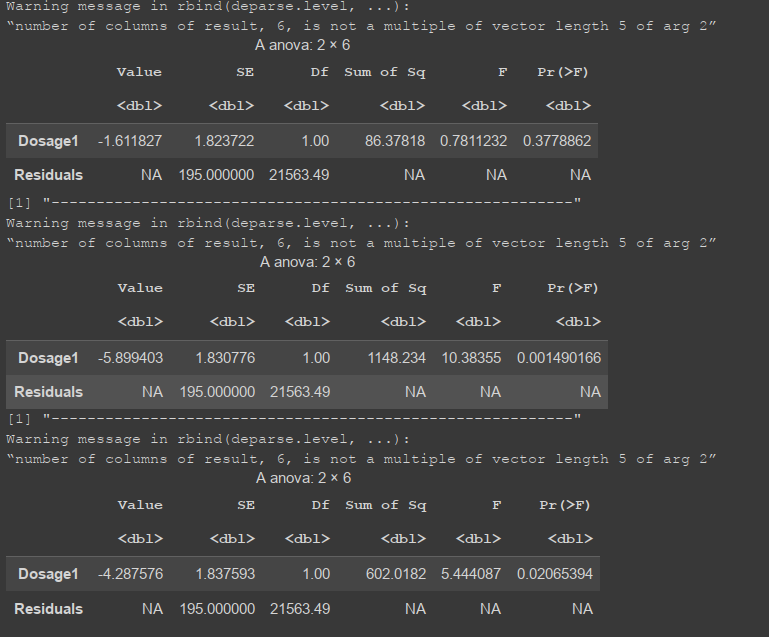
\includegraphics[width=0.8\linewidth]{part01_figures/16.png}
    \caption{Phân tích t-test các nhóm}
    \label{fig:Phân tích t-test các nhóm}
\end{figure}
Với các giả định:
    \begin{itemize}
        \item H0: Không có sự tương tác giữa 2 nhóm thuốc được nhắc đến.
        \item H1: H1: Có sự tương tác giữa 2 nhóm thuốc được nhắc đến
    \end{itemize}
    Với độ tin cậy 0.05, ta có nhận xét như sau:
    \begin{itemize}
        \item Nhóm A và S không có sự tương tác với nhau
        \item Nhóm A và T có sự tương tác với nhau
        \item Nhóm T và S có sự tương tác với nhau
    \end{itemize}

\item \textbf{Bước 3.2: Phân tích ảnh hưởng chính của Drug với hiệu quả của bài kiểm tra trí nhớ}
    \begin{lstlisting}
drug_model = aov(Diff~Drug, data = processed_islander)
summary(drug_model)
    \end{lstlisting}

\newpage
Kết quả:
    \begin{lstlisting}
             Df Sum Sq Mean Sq F value   Pr(>F)    
Drug          2   4305  2152.4   22.71 1.36e-09 ***
Residuals   195  18481    94.8                     
---
Signif. codes:  0 '***' 0.001 '**' 0.01 '*' 0.05 '.' 0.1 ' ' 1
    \end{lstlisting}
Nhận xét: Với mức ý nghĩa 0.05, ta thấy rằng Dosage có ý nghĩa trong việc giải thích mô hình.

\begin{lstlisting}
# Shapiro-Wilk test
av_residual = rstandard(drug_model)
shapiro.test(av_residual)

# Trực quan bằng QQ plot
qqnorm(av_residual)
qqline(av_residual)
hist(av_residual)
\end{lstlisting}
Kết quả:
\begin{lstlisting}
    Shapiro-Wilk normality test

data:  av_residual
W = 0.96098, p-value = 2.777e-05
\end{lstlisting}
\begin{figure}[H]
    \centering
    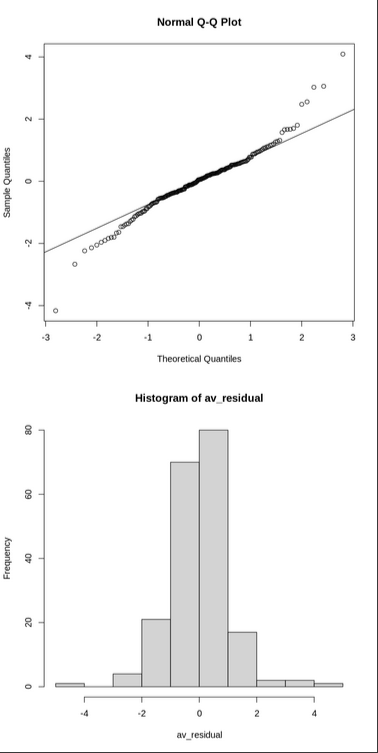
\includegraphics[width=0.5\linewidth]{part01_figures/17.png}
    \caption{Đồ thị phần dư của ảnh hưởng chính giữa Drug và Diff}
    \label{fig:Đồ thị phần dư của ảnh hưởng chính giữa Drug và Diff}
\end{figure}
Với các giả định:
    \begin{itemize}
        \item H0: Phần dư tuân theo phân phối chuẩn.
        \item H1: Phần dư không tuân theo phân phối chuẩn
    \end{itemize}
Nhận xét: với độ tin cậy 5\% thì với giá trị p-value = 2.777e-05 chúng ta đủ cơ sở bác bỏ H0, vậy sai số có phân phối không chuẩn. Nhìn vào biểu đồ, ta thấy rằng ở phần đuôi kéo dài, có một vài điểm bị kéo lệch ra khỏi đường thẳng, Khả năng các điểm nhiễu chính là các điểm ngoại lệ (outliners), tuy nhiên, về mặt tổng quan, dữ liệu vẫn có dạng gần chuẩn.

\newpage
    \begin{lstlisting}
# Kiểm định các nhóm có phương sai đồng nhất hay không
leveneTest(drug_model)
    \end{lstlisting}
Kết quả:
\begin{lstlisting}
A anova: 2 x 3 	
    Df	F value	Pr(>F)
	<int>	<dbl>	<dbl>
group	2	19.06641	2.735522e-08
	195	NA	NA
\end{lstlisting}
Với các giả định:
    \begin{itemize}
        \item H0: Các nhóm có phương sai đồng nhất
        \item H1: Các nhóm không có phương sai đồng nhất
    \end{itemize}
Nhận xét: Với giá trị p-value = 2.735522e-08 < 0.05, ta đủ điều kiện bác bỏ H0, vậy các nhóm có phương sai không đồng nhất.

\begin{lstlisting}
# Kiểm định tính độc lập của phần dư
durbinWatsonTest(drug_model)
plot(drug_model, 1)
\end{lstlisting}

Kết quả:
\begin{lstlisting}
 lag Autocorrelation D-W Statistic p-value
   1       0.2969101      1.398674       0
 Alternative hypothesis: rho != 0
\end{lstlisting}
Với các giả định:
    \begin{itemize}
        \item H0: Không có sự tương quan (độc lập)
        \item H1: Có sự tương quan (không độc lập)
    \end{itemize}
Nhận xét: Với giá trị p-value = 0 nên có sự tương quan dương.
Măc dù với điều kiện phương sai giữa các nhóm không đồng nhất nên sẽ không tiến hành phân
tích ANOVA được, tuy nhiên về mặc trực quan hóa dữ liệu, ta thấy rằng đồ thị phân bố dạng
gần chuẩn, nên ta sẽ tiếp tục đi phân tích các yếu tố ANOVA.

\newpage

\begin{lstlisting}
# Kiểm định độ hiệu quả trung bình giữa các nhóm thuốc
with(processed_islander, pairwise.t.test(Diff, Drug, p.adj = "bonferroni"))
TukeyHSD(aov(Diff~Drug, data=processed_islander), conf.level = 0.95)
plot(TukeyHSD(aov(Diff~Drug, data=processed_islander), conf.level = 0.95))
\end{lstlisting}
Kết quả:
\begin{figure}[H]
    \centering
    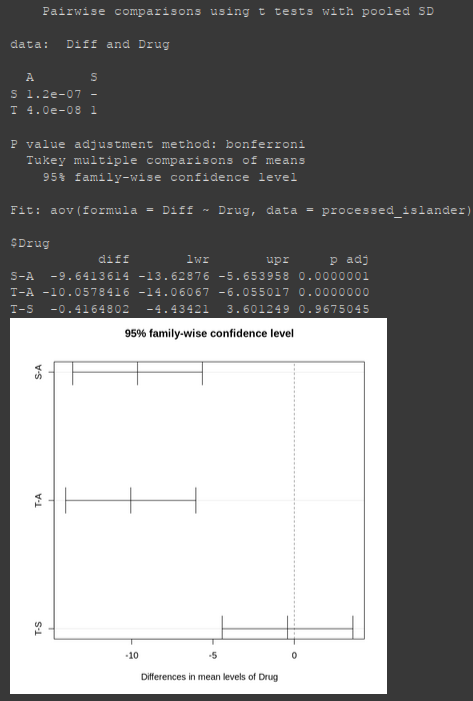
\includegraphics[width=0.7\linewidth]{part01_figures/18.png}
    \caption{Phân tích trung bình giữa các nhóm}
    \label{fig:Phân tích trung bình giữa các nhóm}
\end{figure}
Với các giả thuyết:
    \begin{itemize}
        \item H0: Các giá trị trung bình giữa các cặp bằng nhau
        \item H1: Các giá trị trung bình giữa các cặp không bằng nhau
    \end{itemize}
    Nhìn vào kết quả ta có:
    \begin{itemize}
        \item Nhóm T-S có p-value > 0.05 nên không đủ bác bỏ H0, vậy nhóm này có giá trị trung bình bằng nhau.
        \item Các nhóm còn lại p-value đều có giá trị nhỏ hơn 0.05 (độ tin cậy 95\%) nên ta có cơ sở để bác bỏ H0. Vậy rõ ràng giữa các nhóm nàycó giá trị trung bình là khác nhau. Nghĩa là các nhóm thuốc khác nhau thì cho thấy mức độ ảnh hưởng đến bệnh nhân khác nhau. Nhìn vào kết quả và hình vẽ ta cũng thấy ngay giữa nhóm S-A và T-A có mức độ hiệu quả trung bình khác nhau, T-S có mức độ hiệu quả trung bình như nhau (đồ thị cắt điểm 0)
    \end{itemize}
\end{itemize}
\subsection{Xây dựng và kiểm định mô hình cộng (Additive model)}
\begin{lstlisting}
# Xây dựng mô hình cộng
add_model = lm(Diff~., data=processed_islander)
add_model <- MASS::stepAIC(add_model, k = log(nrow(processed_islander)), trace = 0)
summary(add_model)
\end{lstlisting}
\begin{figure}[H]
    \centering
    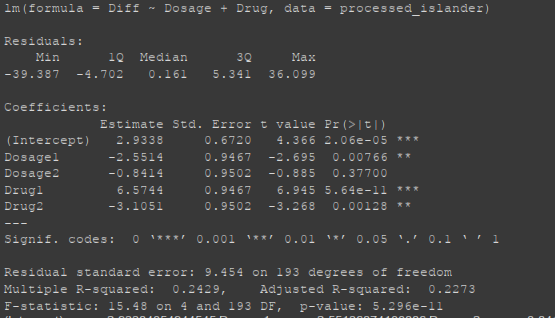
\includegraphics[width=0.8\linewidth]{part01_figures/19.png}
    \caption{Kết quả mô tả của mô hình tuyến tính}
    \label{fig:Kết quả mô tả của mô hình tuyến tính}
\end{figure}

Nhận xét:  Với độ tin cậy 5\%, các biến Dosage và Drug đều có ý nghĩa trong giải thích mô hình. Ta tiến hành kiểm định Shapiro và Breusch-Pagan

\begin{lstlisting}
# Shapiro-Wilk test
av_residual = rstandard(add_model)
shapiro.test(av_residual)

# Trực quan bằng QQ plot
qqnorm(av_residual)
qqline(av_residual)
hist(av_residual)
\end{lstlisting}

Kết quả:
\begin{lstlisting}
    Shapiro-Wilk normality test

data:  av_residual
W = 0.96409, p-value = 6.156e-05
\end{lstlisting}

Với các giả định:
    \begin{itemize}
        \item Phần dư H0: Tuân theo phân phối chuẩn
        \item H1: Phần dư Không tuân theo phân phối chuẩn
    \end{itemize}
Nhận xét: với độ tin cậy 5\% thì với giá trị p-value = 6.156e-05 chúng ta đủ cơ sở bác bỏ H0, vậy sai số có phân phối không chuẩn. Nhìn vào biểu đồ, ta thấy rằng ở phần đuôi kéo dài, có một vài điểm bị kéo lệch ra khỏi đường thẳng --> Khả năng các điểm nhiễu chính là các điểm ngoại lệ (outliners), tuy nhiên, về mặt tổng quan, dữ liệu vẫn có dạng gần chuẩn.

\begin{lstlisting}
# Kiểm định tính độc lập của phần dư
durbinWatsonTest(add_model)
plot(add_model, 1)
\end{lstlisting}

Kết quả:
\begin{lstlisting}
lag Autocorrelation D-W Statistic p-value
   1       0.2550773      1.484015   0.002
Alternative hypothesis: rho != 0
\end{lstlisting}
Với các giả định:
    \begin{itemize}
        \item H0: Không có sự tương quan (độc lập)
        \item H1: Có sự tương quan (không độc lập)
    \end{itemize}
Nhận xét:  Với giá trị p-value = 0.02 < 0.05 nên có sự tương quan dương.

\begin{lstlisting}
# Kiểm định  Breusch-Pagan
bptest(add_model)
\end{lstlisting}
Kết quả:
\begin{lstlisting}
	studentized Breusch-Pagan test

data:  add_model
BP = 9.0739, df = 4, p-value = 0.05928
\end{lstlisting}
Với các giả định:
    \begin{itemize}
        \item H0: phương sai không đổi
        \item H1: phương sai thay đổi
    \end{itemize}
Nhận xét:  Với p-value=0.059 > 0.05 thì ta không đủ điều kiện bác bỏ H0. Vậy phương sai của mô hình không thay đổi.

Như vậy, mô hình cộng được xây dựng như sau:
\[
\text{Diff} = 2.9338 - 2.5514 \times \text{Dosage}_1 - 0.8414 \times \text{Dosage}_2 + 6.5744 \times \text{Drug}_1 - 3.1051 \times \text{Drug}_2
\]
 Với Adjusted R-squared = 0.2273, các biến giải thích được 22,73\% ý nghĩa của mô hình, điều này có nghĩa rằng việc phục hồi trí nhớ sẽ bị chi phối bởi rất nhiều yếu tố (phần lớn là bản thân của ngươi bệnh trầm cảm), chứ không chỉ mỗi tác động của thuốc. Sau đây sẽ là một số nhận xét của mô hình này:
 \begin{itemize}
     \item Hiệu ứng của liều lượng thứ nhất so với mức cơ bản. Giảm thời gian hoàn thành bài kiểm tra trí nhớ xuống 2.5514 giây, có ý nghĩa thống kê (p < 0.01).
     \item Dosage2: Hiệu ứng của liều lượng thứ hai so với mức cơ bản. Giảm thời gian hoàn thành bài kiểm tra trí nhớ xuống 0.8414 giây, nhưng không có ý nghĩa thống kê (p = 0.377).
     \item Drug1: Hiệu ứng của loại thuốc thứ nhất so với mức cơ bản. Tăng thời gian hoàn thành bài kiểm tra trí nhớ lên 6.5744 giây, có ý nghĩa thống kê cao (p < 0.001).
    \item Drug2: Hiệu ứng của loại thuốc thứ hai so với mức cơ bản. Giảm thời gian hoàn thành bài kiểm tra trí nhớ xuống 3.1051 giây, có ý nghĩa thống kê (p < 0.01).
    \item  F-statistic: 15.48 với p-value = 5.296e-11, cho thấy mô hình tổng thể có ý nghĩa thống kê.
 \end{itemize}
 Kết luận: Nếu xem bản thân loại thuốc và liều thuốc tương tác một cách độc lập, thì sau đây là khuyến nghị cho bác sỹ:
 \begin{itemize}
     \item Liều lượng: Liều lượng thứ nhất có ảnh hưởng đáng kể đến thời gian hoàn thành bài kiểm tra trí nhớ, trong khi liều lượng thứ hai không có ảnh hưởng đáng kể. Khuyến nghị bác sỹ dùng liều lượng thứ nhất (liều lượng thấp). 
     \item Loại thuốc: Cả hai loại thuốc đều có ảnh hưởng đáng kể đến thời gian hoàn thành bài kiểm tra trí nhớ, với loại thuốc thứ nhất tăng thời gian và loại thuốc thứ hai giảm thời gian. Khuyến nghị bác sỹ sử cho bệnh nhân sử dụng loại thuốc thứ hai (loại thuốc S)
 \end{itemize}
 Thực tế thì 2 nhân tố này ảnh hưởng trực tiếp đến nhau và cho kết quả khác với mô hình cộng (phân tích ảnh hưởng đơn ở phần trước) vì vậy, cần phải cẩn thận cân nhắc khi sử dụng thuốc tránh đem lại hậu quả không mong muốn ngoài tầm kiểm soát.

 \subsection{Cải tiến mô hình}
 Như chúng ta đã thấy ở các bước phân tích trên, khi phân tích ảnh hưởng chính cũng như xây dựng mô hình tuyến tính, có một số yêu cầu chưa thoả mãn (ví dụ như tính chuẩn, tính độc lập của phương sai), vì vậy, trong phần này chúng ta sẽ tập trung sử lý dữ liệu cho phù hợp hơn. Như đã nhận định ở trên, hiện tại dữ liệu chúng ta đang tồn tại các điểm ngoại lai và cực ngoại lai, trong thí nghiệm này, chúng ta tiến hành loại bỏ các điểm này và tiến hành khảo sát. Ở phần này, tôi sẽ không trình bày chi tiết từng bước như trước (vì các bước thực hiện như nhau, mã thực thi đính kèm); chỉ trình bày những điểm thay đổi chính so với việc phân tích từ tập dữ liệu thô ban đầu.

 Đầu tiên ta sẽ tiến hành khảo sát các điểm ngoại lai bằng lệnh sau

 \begin{lstlisting}
 # Khảo sát ngoại lai theo biến diff
diff_data = processed_islander["Diff"]
outliers_index = list()
extreme_outliers_index = list()

for (i in 1:ncol(diff_data)) {
  # Tính toán Q1, Q3 và IQR
  Q1 = quantile(diff_data[, i], 0.25, na.rm = TRUE)
  Q3 = quantile(diff_data[, i], 0.75, na.rm = TRUE)
  IQR = Q3 - Q1

  # Xác định ngoại lai
  outliers_index_i = diff_data[, i] < (Q1 - 1.5 * IQR) | diff_data[, i] > (Q3 + 1.5 * IQR)
  # outliers_i = diff_data[diff_data[, i] < (Q1 - 1.5 * IQR) | diff_data[, i] > (Q3 + 1.5 * IQR), i]

  # Lưu trữ ngoại lai
  field_name = names(diff_data)[i]
  outliers_index[[field_name]] = which(outliers_index_i)

  # Xác định cực ngoại lai
  extreme_outliers_index_i = diff_data[, i] < (Q1 - 3 * IQR) | diff_data[, i] > (Q3 + 3 * IQR)
  extreme_outliers_index[[field_name]] = which(extreme_outliers_index_i)
}
# In kết quả theo từng biến ra màn hình
for (i in 1:ncol(diff_data)) {
  print(paste("Biến:", names(diff_data)[i]))
  print(paste("Số ngoại lai:", length(outliers_index[[names(diff_data)[i]]])))
  print(paste("Số cực ngoại lai:", length(extreme_outliers_index[[names(diff_data)[i]]])))
}

# Tìm tổng số quan trắc ngoại lai và cực ngoại lai thực sự
outliers = c()
extreme_outliners = c()
for (i in 1:ncol(diff_data)){
    outliers = c(outliers, outliers_index[[names(diff_data)[i]]])
    extreme_outliners = c(extreme_outliners, extreme_outliers_index[[names(diff_data)[i]]])
}

outliers = unique(outliers)
extreme_outliners = unique(extreme_outliners)
print(paste("Tổng số ngoại lai:", length(outliers)))
print(paste("Tổng số cực ngoại lai:", length(extreme_outliners)))
 \end{lstlisting}

\newpage
 Kết quả:
 \begin{lstlisting}
[1] "Biến: Diff"
[1] "Số ngoại lai: 20"
[1] "Số cực ngoại lai: 5"
[1] "Tổng số ngoại lai: 20"
[1] "Tổng số cực ngoại lai: 5"
 \end{lstlisting}

 Như vậy, tổng số ngoại lai và cực ngoại là là 25 samples (chiếm khoảng 12\%). Ta tiến hành loại bỏ các điểm này

 \begin{lstlisting}
# Loại bỏ các điểm ngoại lai và cực ngoại lai
rm_outliner_islander = processed_islander[-extreme_outliners,]
rm_outliner_islander = rm_outliner_islander[-outliers,]

# Kiểm tra lại số lượng dữ liệu
dim(rm_outliner_islander)
str(rm_outliner_islander)
 \end{lstlisting}
Kết quả
\begin{lstlisting}
173 3
'data.frame':	173 obs. of  3 variables:
 $ Dosage: Factor w/ 3 levels "1","2","3": 1 1 1 1 1 1 1 1 1 1 ...
 $ Drug  : Factor w/ 3 levels "A","S","T": 1 1 1 1 1 1 1 1 1 1 ...
 $ Diff  : num  -2.3 -0.9 -4.6 -0.5 0.1 -8.3 11.9 -1.5 -11.2 12 ...
\end{lstlisting}

\newpage
Như vậy, sau khi loại bỏ các điểm ngoại lai ta thu còn lại 173 samples. Ta tiến hành trực quan hoá đồ thị của dữ liệu

\begin{lstlisting}
# Biến phụ thuộc Diff
ggplot(rm_outliner_islander, aes(x = Diff)) +
  geom_histogram(aes(y = ..density..), bins = 30, color = "black", fill = "lightblue") +
  geom_density(alpha = 0.2, fill = "#FF6666") +
  stat_function(fun = dnorm, args = list(mean = mean(rm_outliner_islander$Diff, na.rm = TRUE), sd = sd(rm_outliner_islander$Diff, na.rm = TRUE)),
                color = "blue", size = 1) +
  theme_minimal() +
  labs(title = "Histogram of Diff variable", x = "Diff", y = "Density")
  summary(rm_outliner_islander$Diff)
\end{lstlisting}

Kết quả:
\begin{figure}[H]
    \centering
    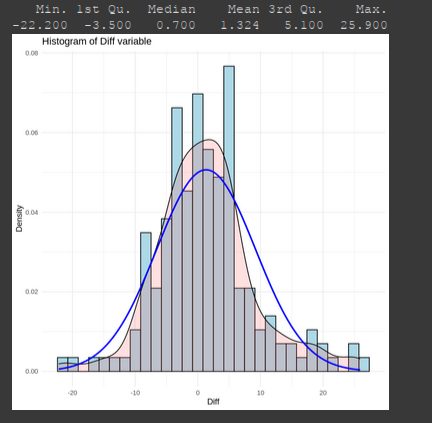
\includegraphics[width=0.7\linewidth]{part01_figures/20.png}
    \caption{Trực quan hóa dữ liệu của biến Diff}
    \label{fig:Trực quan hóa dữ liệu của biến Diff}
\end{figure}

Nhận xét: Sau khi loại bỏ các điểm ngoại lai và cực ngoại lai, ta thu được đồ thị gần chuẩn và có hình dáng tốt hơn trước khi loại.


Tiếp theo chúng ta sẽ tiến hành xây dựng mô hình tương tác và kiểm định các giả thuyết

\begin{lstlisting}
int_model = aov(Diff~ Dosage * Drug, rm_outliner_islander)
\end{lstlisting}

\begin{lstlisting}
# Kiểm định shaoiro test
av_residual = rstandard(int_model)
shapiro.test(av_residual)

# Trực quan bằng QQ plot
qqnorm(av_residual)
qqline(av_residual)
hist(av_residual)
\end{lstlisting}

Kết quả:

\begin{lstlisting}
             Df Sum Sq Mean Sq F value   Pr(>F)    
Dosage        2    190    94.8   2.115    0.124    
Drug          2    957   478.4  10.670 4.40e-05 ***
Dosage:Drug   4   2166   541.6  12.079 1.25e-08 ***
Residuals   164   7354    44.8                     
---
Signif. codes:  0 '***' 0.001 '**' 0.01 '*' 0.05 '.' 0.1 ' ' 1

	Shapiro-Wilk normality test

data:  av_residual
W = 0.98596, p-value = 0.08056
\end{lstlisting}
\begin{figure}[H]
    \centering
    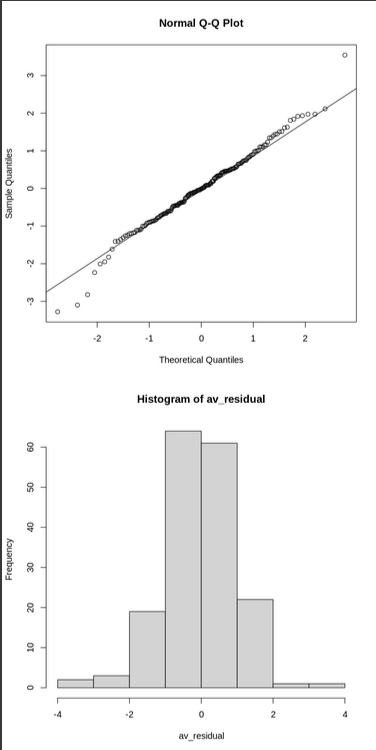
\includegraphics[width=0.7\linewidth]{part01_figures/21.png}
    \caption{Phân phối của phần dư sau khi cải tiến}
    \label{fig:Phân phối của phần dư sau khi cải tiến}
\end{figure}
Với giả định \begin{itemize}
    \item H0: Phần dư tuân theo phân phối chuẩn
    \item H1: Phần dư không tuân theo phân phối chuẩn
\end{itemize}

Với giả độ tin cậy 0.05 thì ta không đủ điều kiện bác bỏ H0, vậy phần dư tuân theo phân phối chuẩn. Măc khác ta thấy rằng thấy bản thân liều lượng (Dosage) sẽ không tác động đến hiệu quả của người sử dụng thuốc, tuy nhiên chúng có mối liên hệ mật thiết (có tương tác) với loại thuốc.
\newpage
Tiếp theo chúng ta đi kiểm định tính độc lập của phần dư:
\begin{lstlisting}
# Kiểm định tính độc lập của phần dư
durbinWatsonTest(int_model)
plot(int_model, 1)
\end{lstlisting}
Kết quả
\begin{lstlisting}
 lag Autocorrelation D-W Statistic p-value
   1      -0.1264805      2.251922   0.304
 Alternative hypothesis: rho != 0
\end{lstlisting}
\begin{figure}[H]
    \centering
    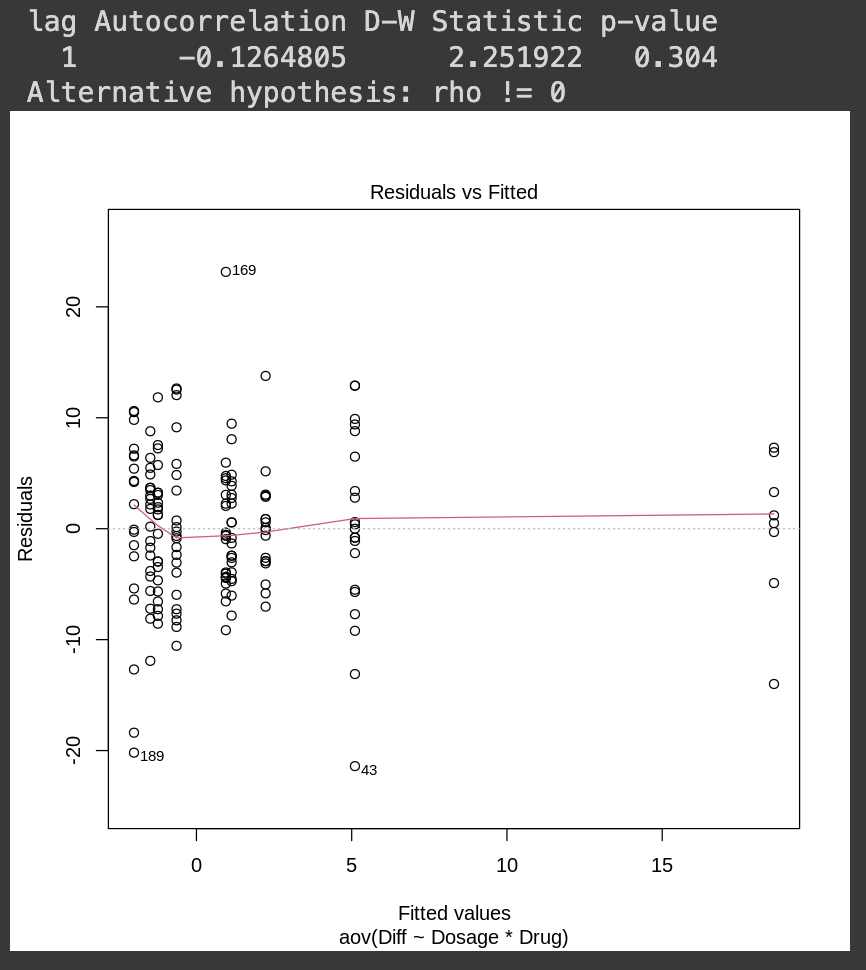
\includegraphics[width=0.8\linewidth]{part01_figures/23.png}
    \caption{Đồ thị  Residuals}
    \label{fig:Đồ thị  Residuals}
\end{figure}
Với mức ý nghĩa 5\%, ta thấy rằng mô hình có phần dư độc lập.
Tiếp tục Kiểm định các nhóm có phương sai đồng nhất hay không

\begin{lstlisting}
# Kiểm định các nhóm có phương sai đồng nhất hay không
leveneTest(int_model)
\end{lstlisting}

Kết quả
\begin{lstlisting}
A anova: 2 x 3
Df	F value	Pr(>F)
<int>	<dbl>	<dbl>
group	8	1.440304	0.1833148
164	NA	NA

\end{lstlisting}

Với mức ý nghĩa 5\%, ta thấy mô hình có phương sai của các nhóm đồng nhất. Như vậy, ta đủ điều kiện để phân tích ANOVA. Bước tiếp theo, chúng ta sẽ tiến hành kiểm tra tương tác đơn và tương tác chính như phần trước.

\begin{itemize}
    \item \textbf{Bước 1: Kiểm tra sự tương tác }
    \begin{lstlisting}
summary(int_model)
plot(interactionMeans(int_model))
    \end{lstlisting}

Kết quả:
\begin{figure}[H]
    \centering
    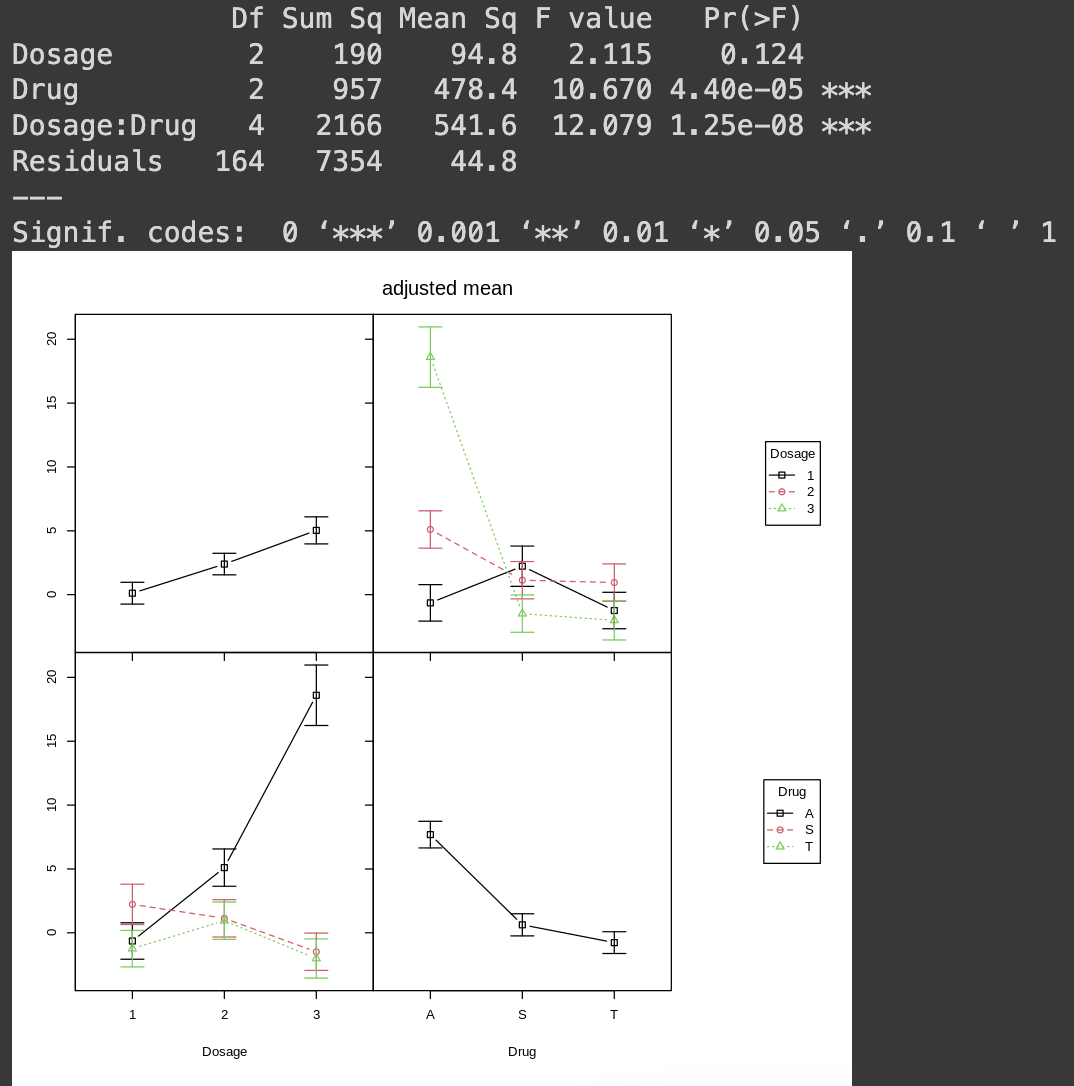
\includegraphics[width=0.7\linewidth]{part01_figures/24.png}
    \caption{Tương tác giữa Drug và Dosage}
    \label{fig:Tương tác giữa Drug và Dosage}
\end{figure}
Nhận xét: Với mức ý nghĩa 5\%, ta thấy giữa `Dosage` và `Drug` có sự tương tác với nhau (p-value=1.25e-08). Sự kết hợp giữa hàm lượng thuốc và loại thuốc có ảnh hưởng rất lớn đến thời gian hoàn thành bài kiểm tra, cho thấy rằng không chỉ từng yếu tố riêng lẻ mà sự kết hợp giữa chúng cũng rất quan trọng. Về phần nhận xét chi tiết xem lại phần đầu tiên vì kết quả biểu đồ giống với phân tích của phần đầu.

    \item \textbf{Bước 2: Phân tích ảnh hưởng đơn}
    \begin{itemize}
        \item[a.] \textbf{Phân tích ảnh hưởng đơn của liều lượng ở mỗi loại thuốc}
        \begin{lstlisting}
testInteractions(int_model, fixed = "Drug", across = "Dosage")
        \end{lstlisting}
    Kết quả:
    \begin{figure}[H]
        \centering
        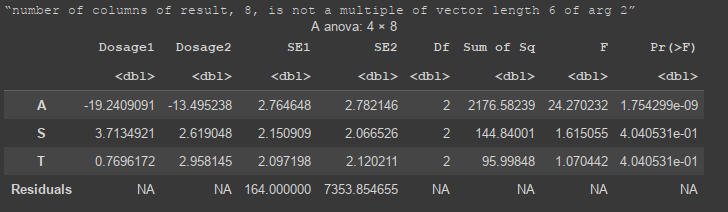
\includegraphics[width=0.8\linewidth]{part01_figures/25.png}
        \caption{Kết quả ảnh hưởng đơn của liều lượng ở mỗi loại thuốc}
        \label{fig:Kết quả ảnh hưởng đơn của liều lượng ở mỗi loại thuốc}
    \end{figure}
    Giả định:
        \begin{itemize}
            \item H0: Liều lượng Không ảnh hưởng đến hiệu quả thuốc
            \item H1: Liều lượng Có ảnh hưởng đến hiệu quả của thuốc
        \end{itemize}
    Nhận xét: Với kết quả phân tích ta có một số nhận xét như sau, với độ tin cậy 5\% thì:
        \begin{itemize}
            \item Liều lượng có ảnh hưởng đến kết quả của loại thuốc A
            \item Liều lượng không ảnh hưởng đến kết quả của lọai thuốc S và T
        \end{itemize}
    \item [b].\textbf{ Phân tích ảnh hưởng đơn của thuốc ở mỗi liều lượng}
        \begin{lstlisting}
testInteractions(int_model, fixed = "Dosage", across = "Drug")
        \end{lstlisting}
        \newpage
        Kết quả:
        \begin{figure}[H]
            \centering
            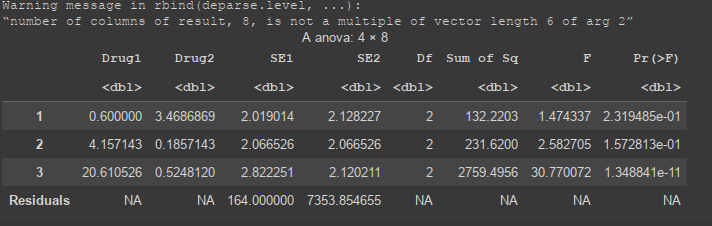
\includegraphics[width=0.8\linewidth]{part01_figures/26.png}
            \caption{Kết quả ảnh hưởng đơn của thuốc ở mỗi liều lượng}
            \label{fig:Kết quả ảnh hưởng đơn của thuốc ở mỗi liều lượng}
        \end{figure}
        Với giả định
        \begin{itemize}
            \item H0: Các loại thuốc sẽ không tác động ở mỗi liều lượng
            \item H1: Các loại thuốc sẽ có tác động ở mỗi liều lượng
        \end{itemize}
        Nhận xét: Với kết quả phân tích ta có một số nhận xét như sau, với độ tin cậy 5\% thì: Hầu hết các loại thuốc sẽ có tác động ở liều lượng cao; liều lượng thấp và trung bình cho kết quả không đáng kể.
         \item [c.] \textbf{Phân tích ảnh hưởng đơn giữa các nhóm thuốc ứng với mỗi liều lượng}
        \begin{lstlisting}
options(contrasts = c(unordered="contr.sum", ordered="contr.poly"))
A_vs_S = list(Drug = c(1, -1, 0))
A_vs_T = list(Drug = c(1, 0, -1))
S_vs_T = list(Drug = c(0, 1, -1))
# Nhóm A và S
testInteractions(int_model, custom = c(A_vs_S), fixed = "Dosage", adjustment = "bonferroni")
        \end{lstlisting}
    \begin{figure}[H]
            \centering
            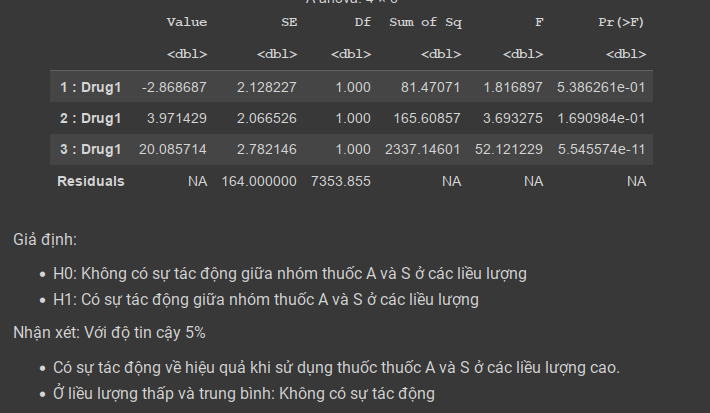
\includegraphics[width=0.7\linewidth]{part01_figures/27.png}
            \caption{Ảnh hưởng giữa nhóm A và S}
            \label{fig:Ảnh hưởng giữa nhóm A và S}
        \end{figure}
                
        Với các giả định:
        \begin{itemize}
            \item H0: Không có sự tác động giữa nhóm thuốc A và S ở các liều lượng
            \item H1: Có sự tác động giữa nhóm thuốc A và S ở các liều lượng
        \end{itemize}
        Nhận xét: Với độ tin cậy 5\% Có sự tác động về hiệu quả khi sử dụng thuốc thuốc A và S ở các liều lượng cao.Ở liều lượng thấp và trung bình: Không có sự tác động.

    \begin{lstlisting}
# Nhóm A và T
testInteractions(int_model, custom = c(A_vs_T), fixed = "Dosage", adjustment = "bonferroni")
    \end{lstlisting}
    \begin{figure}[H]
        \centering
        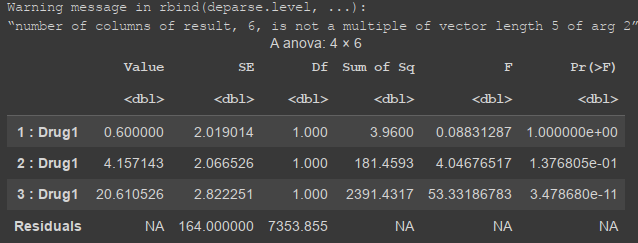
\includegraphics[width=0.7\linewidth]{part01_figures/28.png}
        \caption{Ảnh hưởng giữa nhóm A và T}
        \label{fig:Ảnh hưởng giữa nhóm A và T}
    \end{figure}
    
    Với các giả định:
        \begin{itemize}
            \item H0: Không có sự tác động giữa nhóm thuốc A và T ở các liều lượng
            \item H1: Có sự tác động giữa nhóm thuốc A và T ở các liều lượng
        \end{itemize}
        Nhận xét: Với độ tin cậy 5\% Có sự tác động về hiệu quả khi sử dụng thuốc thuốc A và T ở các liều lượng cao.Ở liều lượng thấp và trung bình: Không có sự tác động.

    \begin{lstlisting}
# Nhóm S và T
testInteractions(int_model, custom = c(S_vs_T), fixed = "Dosage", adjustment = "bonferroni")
    \end{lstlisting}
    <chèn ảnh>
    \begin{figure}[H]
            \centering
            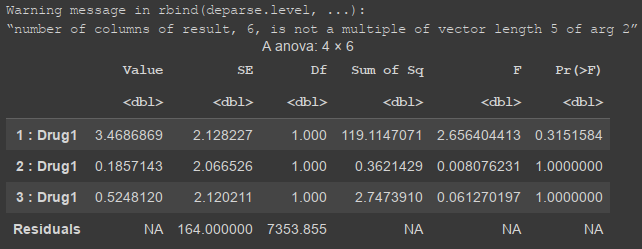
\includegraphics[width=0.8\linewidth]{part01_figures/29.png}
            \caption{Ảnh hưởng giữa S và T}
            \label{fig:Ảnh hưởng giữa S và T}
        \end{figure}
                Với các giả định:
        \begin{itemize}
            \item H0: Không có sự tác động giữa nhóm thuốc S và T ở các liều lượng
            \item H1: Có sự tác động giữa nhóm thuốc S và T ở các liều lượng
        \end{itemize}
        Nhận xét: Với độ tin cậy 5\% thì không có sự khác biệt nào ở cả 3 liều lượng.
    \item [d.] \textbf{Phân tích ảnh hưởng đơn giữa các nhóm liều lượng ứng với mỗi loại thuốc}
        \begin{lstlisting}
ptions(contrasts = c(unordered="contr.sum", ordered="contr.poly"))
low_vs_medium = list(Dosage = c(1, -1, 0))
low_vs_high = list(Dosage = c(1, 0, -1))
medium_vs_high = list(Dosage = c(0, 1, -1))
        \end{lstlisting}

        \begin{lstlisting}
# Nhóm thấp và trung bình
testInteractions(int_model, custom = c(low_vs_medium), fixed = "Drug", adjustment = "bonferroni")
        \end{lstlisting}
        Kết quả:
        \begin{figure}[H]
            \centering
            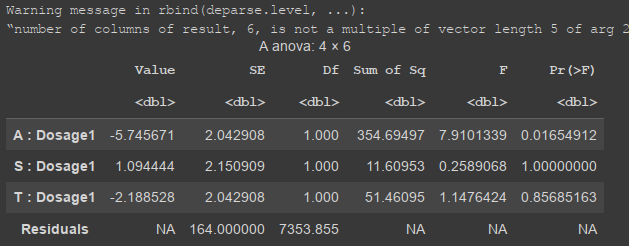
\includegraphics[width=0.8\linewidth]{part01_figures/30.png}
            \caption{Ảnh hưởng giữa nhóm thấp và trung bình}
            \label{fig:Ảnh hưởng giữa nhóm thấp và trung bình}
        \end{figure}

        Với các giả định:
        \begin{itemize}
            \item H0: Không có sự tương tác nhau giữa liều thấp và liều trung bình
            \item H1: Có sự tương tác nhau giữa liều thấp và liều trung bình
        \end{itemize}
        Nhận xét: Với độ tin cậy 5\% Ở loại thuốc A: Có sự tương tác về hiệu quả khi sử dụng thuốc ở các liều lượng thấp và liều lượng trung bình; Ở loại thuốc S và T: Không có sự tương tác có ý nghĩa thống kê.
    \begin{lstlisting}
# Nhóm thấp và cao
testInteractions(int_model, custom = c(low_vs_high), fixed = "Drug", adjustment = "none")
    \end{lstlisting}
    Kết quả:
    \begin{figure}[H]
        \centering
        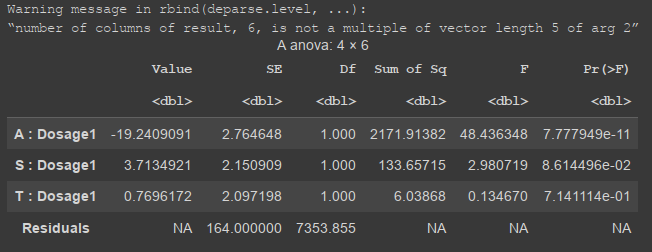
\includegraphics[width=0.8\linewidth]{part01_figures/31.png}
        \caption{Ảnh hưởng giữa nhóm thấp và cao}
        \label{fig:Ảnh hưởng giữa nhóm thấp và cao}
    \end{figure}
    Với các giả định:
        \begin{itemize}
            \item H0: Không có tương tác nhau giữa liều thấp và liều cao
            \item H1: Có tương tác nhau giữa liều thấp và liều cao
        \end{itemize}
    Nhận xét: Với độ tin cậy 5\% Ở loại thuốc A: Có sự tương tác về hiệu quả khi sử dụng thuốc ở các liều lượng thấp và liều lượng cao; Ở loại thuốc S và T: Không có sự tương tác có ý nghĩa thống kê.
    \begin{lstlisting}
# Nhóm trung bình và cao
testInteractions(int_model, custom = c(medium_vs_high), fixed = "Drug", adjustment = "none")
    \end{lstlisting}
    Kết quả:
    \begin{figure}[H]
        \centering
        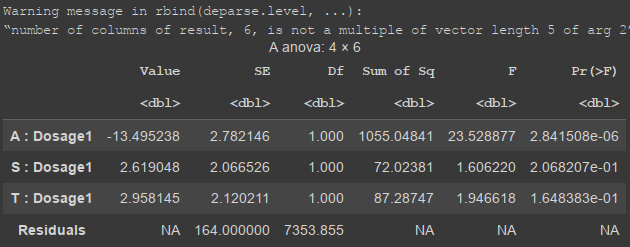
\includegraphics[width=0.8\linewidth]{part01_figures/32.png}
        \caption{Tương tác giữa nhóm trung bình vào cao}
        \label{fig:Tương tác giữa nhóm trung bình vào cao}
    \end{figure}
    
    Với các giả định:
        \begin{itemize}
            \item H0: Không có sự tương tác giữa liều trung bình và liều cao
            \item Có sự tương tác giữa liều trung bình và liều cao
        \end{itemize}
    Nhận xét: Với độ tin cậy 5\% Ở loại thuốc A: Có sự tương tác về hiệu quả khi sử dụng thuốc ở các liều lượng trung bình và liều lượng cao; Ở loại thuốc S và T: Không có sự tương tác có ý nghĩa thống kê.
    
    \item \textbf{Kết luận}: \textbf{Kết quả này giống với kết quả phân tích trước đó. Tuy nhiên các tính chất kiểm định về chuẩn cho đánh giá ANOVA đã cho kết quả tốt hơn so với trước khi chưa xử lý dữ liệu.}
    \end{itemize}
   \item \textbf{Bước 3. Phân tích ảnh hưởng chính}
   \begin{itemize}
       \item \textbf{Phân tích ảnh hưởng chính của Dosage với hiệu quả của bài kiểm tra trí nhớ}
       \begin{lstlisting}
dosage_model = aov(Diff~Dosage, data = rm_outliner_islander)
summary(dosage_model)
       \end{lstlisting}
       Kết quả:
       \begin{lstlisting}
             Df Sum Sq Mean Sq F value Pr(>F)
Dosage        2    190   94.84   1.539  0.218
Residuals   170  10477   61.63               
       \end{lstlisting}
    Nhận xét: Với mức ý nghĩa 0.05, ta thấy rằng Dosage không có ý nghĩa trong việc giải thích mô hình. Theo nguyên tắc thì ta không cần phải đi kiểm định các giả thuyết cho biến này. Tuy nhiên chúng ta vẫn kiểm định để xem kết quả cải thiện như thế nào so với trước đó.
    \begin{lstlisting}
# Shapiro-Wilk test
av_residual = rstandard(dosage_model)
shapiro.test(av_residual)

# Trực quan bằng QQ plot
qqnorm(av_residual)
qqline(av_residual)
hist(av_residual)
    \end{lstlisting}
    Kết quả:
    \begin{lstlisting}
	Shapiro-Wilk normality test
data:  av_residual
W = 0.96742, p-value = 0.0004441
    \end{lstlisting}

    \begin{figure}[H]
        \centering
        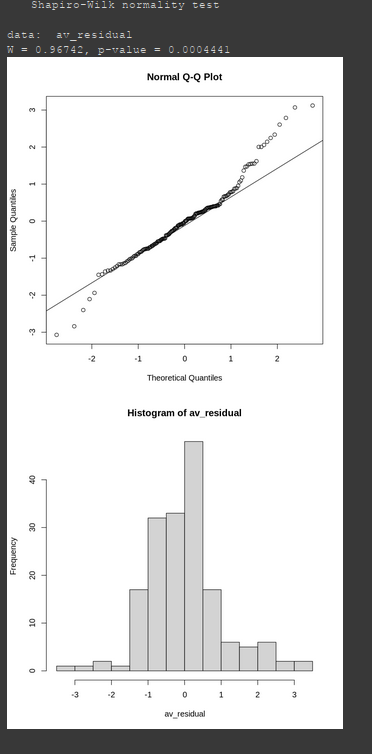
\includegraphics[width=0.6\linewidth]{part01_figures/33.png}
        \caption{Shapiro-test}
        \label{fig:Shapiro-test}
    \end{figure}

    Nhận xét: Giá trị p-value đã tăng lên rất nhiều (mặc dù < 0.05), hình dáng đồ thị gần chuẩn hơn so với trước khi chưa xử lý dữ liệu.
   \end{itemize}
    \begin{lstlisting}
# Kiểm định các nhóm có phương sai đồng nhất hay không
leveneTest(dosage_model)
    \end{lstlisting}
    Kết quả:
    \begin{lstlisting}
A anova: 
2 x 3 	Df	F value	Pr(>F)
	<int>	<dbl>	<dbl>
group	2	4.442547	0.01316301
	170	NA	NA
    \end{lstlisting}
    Nhận xét:
    Với các giả định:
        \begin{itemize}
            \item Các nhóm có phương sai đồng nhất
            \item Các nhóm không có phương sai đồng nhất
        \end{itemize}
    Nhận xét:Với giá trị p-value = 0.013 > 0.05, ta không điều kiện bác bỏ H0, vậy các nhóm có phương sai đồng nhất (trước đó là không đồng nhất) trước đó điều kiện  này không thỏa mãn.
    \begin{lstlisting}
# Kiểm định tính độc lập của phần dư
durbinWatsonTest(dosage_model)
plot(dosage_model, 1)
    \end{lstlisting}
    Kết quả:
    \begin{figure}[H]
        \centering
        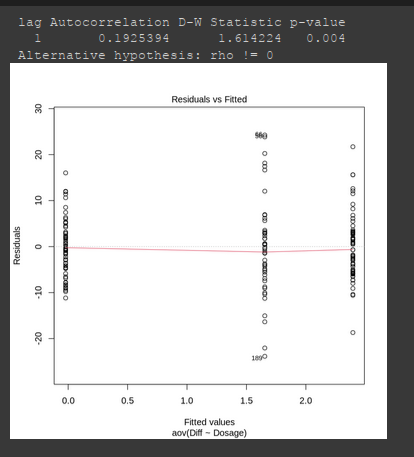
\includegraphics[width=0.8\linewidth]{part01_figures/34.png}
        \caption{Kiểm định độc lập phần dư}
        \label{fig:Kiểm định độc lập phần dư_}
    \end{figure}
        Nhận xét:
    Với các giả định:
        \begin{itemize}
            \item H0: Không có sự tương quan (độc lập)
            \item H1: Có sự tương quan (không độc lập)
        \end{itemize}
    Nhận xét:Với giá trị p-value = 0.02 nên có sự tương quan dương, tuy nhiên kết quả này lớn hơn kết quả trước đó (=0).
    \begin{lstlisting}
# Kiểm định trung bình giữa các nhóm liều lượng
with(rm_outliner_islander, pairwise.t.test(Diff, Dosage, p.adj = "bonferroni"))
TukeyHSD(aov(Diff~Dosage, data=rm_outliner_islander), conf.level = 0.95)
plot(TukeyHSD(aov(Diff~Dosage, data=rm_outliner_islander), conf.level = 0.95))
    \end{lstlisting}
    Kết quả:
    \begin{figure}[H]
        \centering
        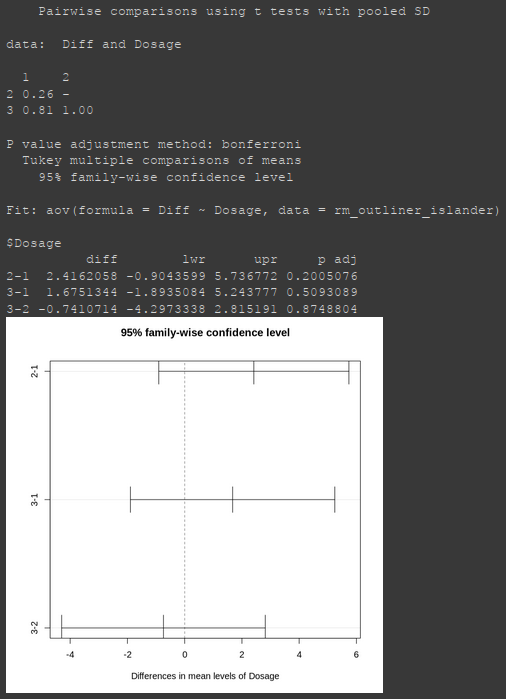
\includegraphics[width=0.8\linewidth]{part01_figures/35.png}
        \caption{Kiểm định trung bình}
        \label{fig:Kiểm định trung bình_}
    \end{figure}

    Với các giả định:
        \begin{itemize}
            \item H0: Các giá trị trung bình giữa các cặp bằng nhau
            \item H1: Các giá trị trung bình giữa các cặp không bằng nhau
        \end{itemize}
    Nhận xét:Các cặp có p-value đều có giá trị lớn hơn 0.05 (độ tin cậy 95\%) nên ta cơ sở để bác bỏ H0. Vậy rõ ràng giữa các nhóm này có giá trị trung bình là như nhau.Để rõ hơn, ta tiến hành kiểm định Tukey's. Nhìn vào kết quả và hình vẽ ta cũng thấy ngay mức độ hiệu quả trung bình như nhau ở 3 nhóm(đồ thị cắt điểm 0). \textbf{Kết quả trước đó cho ta thấy rằng  3-2 và 1-2 có mức độ hiệu quả trung bình như nhau  và 3-1 là khác nhau.}

    \begin{lstlisting}
# ttest
A_vs_S = list(Dosage = c(1, -1, 0))
A_vs_T = list(Dosage = c(1, 0, -1))
S_vs_T = list(Dosage = c(0, 1, -1))
testInteractions(dosage_model, custom = A_vs_S, adjustment = 'bonferroni')
print("----------------------------------------------------------")
testInteractions(dosage_model, custom = A_vs_T, adjustment = 'bonferroni')
print("----------------------------------------------------------")
testInteractions(dosage_model, custom = S_vs_T, adjustment = 'bonferroni')
    \end{lstlisting}
\begin{figure}[H]
    \centering
    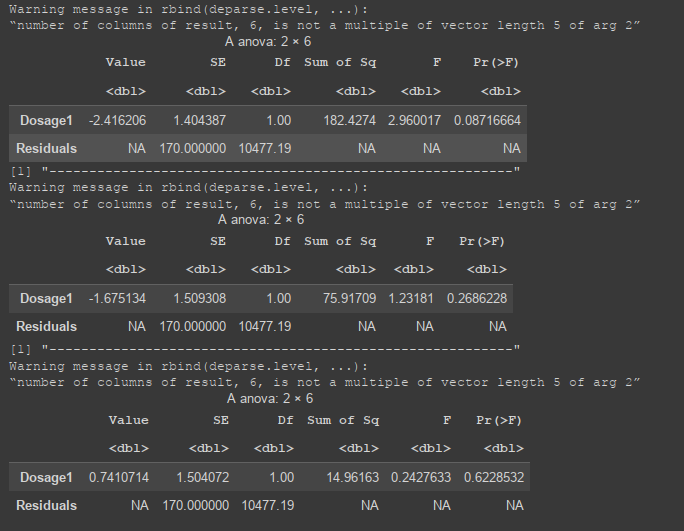
\includegraphics[width=0.8\linewidth]{part01_figures/36.png}
    \caption{Kết quả t-test}
    \label{fig:Kết quả t-test}
\end{figure}
    
    Với các giả định:
    \begin{itemize}
        \item H0: Không có sự tương tác giữa 2 nhóm thuốc được nhắc đến
        \item H1: Có sự tương tác giữa 2 nhóm thuốc được nhắc đến
    \end{itemize}
    Nhận xét: Với p-value=0.05, ta có kết luận như sau: cả 3 nhóm đều có sự tương tác mang ý nghĩa thống kê (giống kết quả trước đó).

    \item \textbf{Phân tích ảnh hưởng chính của Drug với hiệu quả của bài kiểm tra trí nhớ}
    \begin{lstlisting}
drug_model = aov(Diff~Drug, data = rm_outliner_islander)
summary(drug_model)
    \end{lstlisting}
    Kết quả:
    \begin{lstlisting}
             Df Sum Sq Mean Sq F value   Pr(>F)    
Drug          2    896   447.8   7.791 0.000579 ***
Residuals   170   9771    57.5                     
---
Signif. codes:  0 '***' 0.001 '**' 0.01 '*' 0.05 '.' 0.1 ' ' 1
    \end{lstlisting}
    Nhận xét: Với mức ý nghĩa 0.05, ta thấy rằng Drug có ý nghĩa trong việc giải thích mô hình.
    \begin{lstlisting}
# Shapiro-Wilk test
av_residual = rstandard(drug_model)
shapiro.test(av_residual)

# Trực quan bằng QQ plot
qqnorm(av_residual)
qqline(av_residual)
hist(av_residual)
    \end{lstlisting}

    Kết quả:
    \begin{lstlisting}
	Shapiro-Wilk normality test

data:  av_residual
W = 0.9859, p-value = 0.07921
    \end{lstlisting}

    \begin{figure}
        \centering
        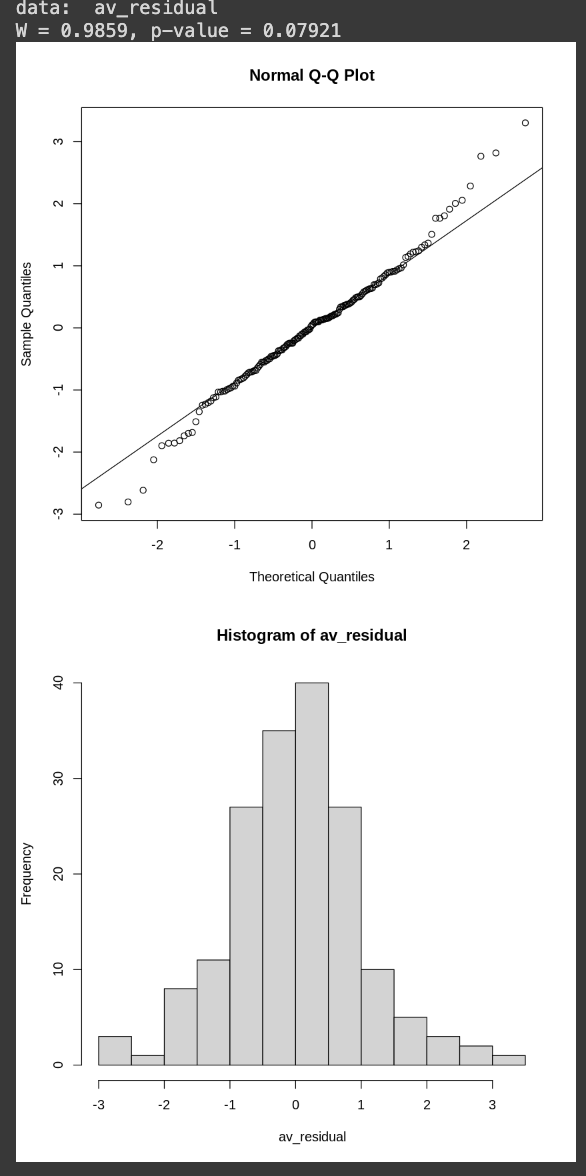
\includegraphics[width=0.5\linewidth]{part01_figures/38.png}
        \caption{Shapiro-Wilk test và đồ thị phần dư}
        \label{fig:Shapiro-Wilk test và đồ thị phần dư}
    \end{figure}

    Với các giả định:
    \begin{itemize}
        \item H0: Tuân theo phân phối chuẩn
        \item H1: Không tuân theo phân phối chuẩn
    \end{itemize}
    Nhận xét: với độ tin cậy 5\% thì với giá trị p-value =0.07921 chúng ta không đủ cơ sở bác bỏ H0, vậy sai số có phân phối chuẩn. Nhìn vào biểu đồ, ta thấy rằng ở phần đuôi kéo dài, có một vài điểm bị kéo lệch ra khỏi đường thẳng về mặt tổng quan, dữ liệu vẫn có dạng gần chuẩn (trước đó là không chuẩn)

    \begin{lstlisting}
# Kiểm định các nhóm có phương sai đồng nhất hay không
leveneTest(drug_model)
    \end{lstlisting}
    Kết quả:
    \begin{lstlisting}
A anova: 
2 x 3 	Df	F value	Pr(>F)
	<int>	<dbl>	<dbl>
group	2	11.12926	2.87001e-05
	170	NA	NA
    \end{lstlisting}
    Với các giả định:
    \begin{itemize}
        \item H0: Các nhóm có phương sai đồng nhất
        \item H1: Các nhóm không có phương sai đồng nhất
    \end{itemize}
    Nhận xét: Nhận xét: Với giá trị p-value = 2.87001e-05 < 0.05, ta đủ điều kiện bác bỏ H0, vậy các nhóm có phương sai không đồng nhất, tuy nhiên kết quả có giá trị p-value cao hơn trước (2.735522e-08).
\begin{lstlisting}
# Kiểm định tính độc lập của phần dư
durbinWatsonTest(drug_model)
plot(drug_model, 1)
\end{lstlisting}
\begin{figure}
    \centering
    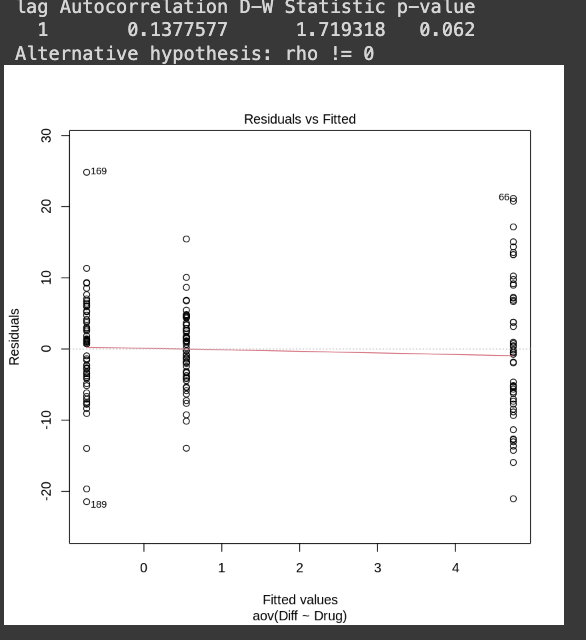
\includegraphics[width=0.8\linewidth]{part01_figures/37.png}
    \caption{Kiểm định tính độc lập của phần dư}
    \label{fig:Kiểm định tính độc lập của phần dư__}
\end{figure}
    Với các giả định:
    \begin{itemize}
        \item H0: Không có sự tương quan (độc lập)
        \item H1: Có sự tương quan (không độc lập)
    \end{itemize}
    Nhận xét: Với giá trị p-value = 0.062 nên không có sự tương quan (trước đó là tương quan dương).

\begin{lstlisting}
# Kiểm định độ hiệu quả trung bình giữa các nhóm thuốc
with(rm_outliner_islander, pairwise.t.test(Diff, Drug, p.adj = "bonferroni"))
TukeyHSD(aov(Diff~Drug, data=rm_outliner_islander), conf.level = 0.95)
plot(TukeyHSD(aov(Diff~Drug, data=rm_outliner_islander), conf.level = 0.95))
\end{lstlisting}
    Với các giả định:
    \begin{itemize}
        \item H0: Các giá trị trung bình giữa các cặp bằng nhau
        \item H1: Các giá trị trung bình giữa các cặp không bằng nhau
    \end{itemize}
    Nhận xét: \begin{itemize}
        \item Nhìn vào kết quả ta có: Nhóm T-S có p-value > 0.05 nên không đủ bác bỏ H0, vậy nhóm này có giá trị trung bình bằng nhau; Các nhóm còn lại p-value đều có giá trị nhỏ hơn 0.05 (độ tin cậy 95\%) nên ta có cơ sở để bác bỏ H0. Vậy rõ ràng giữa các nhóm này có giá trị trung bình là khác nhau.
        \item Nhìn vào kết quả và hình vẽ ta cũng thấy ngay giữa nhóm S-A và T-A có mức độ hiệu quả trung bình khác nhau, T-S có mức độ hiệu quả trung bình như nhau (đồ thị cắt điểm 0) (giống kết quả phân tích trước đó).
        \item \textbf{Kết luận}: \textbf{các tính chất kiểm định về chuẩn cho đánh giá ANOVA và kiểm định ảnh hưởng chính đã cho kết quả tốt hơn so với trước khi chưa xử lý dữ liệu.}
    \end{itemize}
    \item \textbf{Bước 4: Xây dựng và kiểm định mô hình cộng (Additive model)}
    \begin{lstlisting}
add_model = lm(Diff~., data=rm_outliner_islander)
add_model <- MASS::stepAIC(add_model, k = log(nrow(rm_outliner_islander)), trace = 0)
summary(add_model)
add_model$coefficients
    \end{lstlisting}
    Kết quả:
    \begin{lstlisting}

Call:
lm(formula = Diff ~ Drug, data = rm_outliner_islander)

Residuals:
     Min       1Q   Median       3Q      Max 
-21.4645  -4.4450   0.3569   4.3550  24.8355 

Coefficients:
            Estimate Std. Error t value Pr(>|t|)    
(Intercept)   1.5176     0.5785   2.623 0.009502 ** 
Drug1         3.2256     0.8428   3.827 0.000182 ***
Drug2        -0.9726     0.8087  -1.203 0.230799    
---
Signif. codes:  0 '***' 0.001 '**' 0.01 '*' 0.05 '.' 0.1 ' ' 1

Residual standard error: 7.581 on 170 degrees of freedom
Multiple R-squared:  0.08396,	Adjusted R-squared:  0.07318 
F-statistic: 7.791 on 2 and 170 DF,  p-value: 0.000579

(Intercept)
    1.51755112797807
Drug1
    3.22558612692389
Drug2
    -0.972551127978073

    \end{lstlisting}
    Nhận xét: Với p-value=5\%, chỉ có biến Drug có ý nghĩ trong việc giải thích mô hình. như vậy việc kiểm định mô hình cộng giống như phân tích ảnh hưởng chính của biến Drug

Như vậy, mô hình cộng được xây dựng như sau:

\textbf{Diff=1.517 + 3.225×Drug1 - 0.972×Drug2}

- Drug1: Hệ số cho Drug1 là 3.2256. Điều này cho thấy rằng khi sử dụng loại thuốc thứ nhất, sự khác biệt trong thời gian hoàn thành bài kiểm tra tăng thêm
3.2256 iây so với không sử dụng thuốc. Hệ số này có ý nghĩa thống kê (p-value = 0.000182 < 0.001)
- Drug2:Hệ số cho Drug2 là -0.9726. Điều này cho thấy rằng khi sử dụng loại thuốc thứ hai, sự khác biệt trong thời gian hoàn thành bài kiểm tra giảm đi
0.9726 giây so với không sử dụng thuốc. Tuy nhiên, hệ số này không có ý nghĩa thống kê (p-value = 0.230799 > 0.05).
- Mô hình tổng thể có ý nghĩa: F-statistic cho thấy mô hình tổng thể có ý nghĩa thống kê, tuy nhiên, Multiple R-squared thấp cho thấy mô hình chỉ giải thích được một phần nhỏ sự biến thiên của Diff

Kết luận: Nếu xem bản thân loại thuốc và liều thuốc tương tác một cách độc lập, thì sau đây là khuyến nghị cho bác sỹ:
Nên sử dụng loại thuốc 2 (thuốc S) cho bệnh nhân.
Thực tế thì việc sử dụng thuốc cần đánh giá ở nhiều khía cạnh (ví dụ như phân tích ảnh hưỏng đơn cho thấy tương tác mạnh với liều lượng) Vì vậy, cần phải cẩn thận cân nhắc khi sử dụng thuốc tránh đem lại hậu quả không mong muốn ngoài tầm kiểm soát.

\textbf{Như vậy về tổng thể sao khi loại bỏ các điểm ngoại lai và cực ngoại lai, về vieeck thống kê và phân tích ANOVA đã cho ra một mô hình có các yếu tố thỏa mãn các yếu tố kiểm định về chuẩn hơn, trong TH không chuẩn nhưng chỉ số so với trước là tốt hơn}
\end{itemize}
